\chapter{Belebtheit} \label{chapter:belebtheit}

Wie in Abschnitt \ref{sec:extension} bereits angesprochen wurde, liegt der vorliegenden Arbeit  die Hypothese zugrunde, dass die Kontextexpansion \is{Expansion} des Definitartikels \is{Definitartikel} von der kognitiv-linguistischen Kategorie \isi{Belebtheit} determiniert wird. Das vorliegende Kapitel leitet diese Hypothese theoretisch her. Nachdem in Abschnitt \ref{sec:belebt} die wichtigsten Belebtheitshierarchien \is{Belebtheitshierarchie} aus der Forschung erläutert werden, diskutiert Abschnitt \ref{sec:belebtwandel}, warum ein belebtheitsgesteuerter \is{Belebtheit} Wandel wahrscheinlich ist. In Abschnitt \ref{sec:indi} wird für eine Erweiterung der Belebtheitsgrundstufen um die Kategorie der \isi{Individualität} argumentiert. Abschnitt \ref{sec:andere-kog} legt offen, mit welchen semantischen Rollen \is{Semantische Rolle} die \isi{Belebtheit} korreliert und inwiefern der Faktor \isi{Relevanz} mit der \isi{Belebtheit} zusammenhängt. Die Zusammenfassung in \ref{sec:bel-zusammenfassung} liefert ein erweitertes Belebtheitsmodell, das die besprochenen Faktoren abbildet. Es wird davon ausgegangen, dass die Entwicklung des Definitartikels \is{Definitartikel} bei \is{Belebtheit} belebten, \is{Individualität} individuierten, \is{Agentivität} agentiven und diskursrelevanten Referenten beginnt und sich von da aus zu anderen Referenten ausbreitet. 

\section{Belebtheitshierarchien}\label{sec:belebt}

Unter \isi{Belebtheit} versteht die Sprachtypologie eine extra-linguistische Hierarchisierung \is{Belebtheitshierarchie} bestehend aus den Hauptkategorien \textsc{menschlich > belebt > unbelebt}, die grammatische Regularitäten, etwa \is{Kasus} Kasus- und Numerusmarkierungen \is{Numerus} oder \is{Wortstellung} Wortstellungsabfolgen, determiniert.\footnote{Weiterführend:  \cite{Silverstein1976,Allan1987,Comrie1989,Langacker1991,Dahl1996,Yamamoto1999,Yamamoto2006,Croft1995,Croft2006,Dixon1995, Corbett2000,Aissen2003,Zifonun2006, Dahl2008}.} In vielen australischen Sprachen werden beispielsweise Akkusative \is{Kasus} nur dann formal markiert, wenn sie auf belebte \is{Belebtheit} Referenten verweisen \parencite[189]{Comrie1989}. 
Im Nhd. stehen belebte \is{Belebtheit} Referenten häufiger an der Spitze des Mittelfeldes \is{Wortstellung} als unbelebte \is{Belebtheit} \parencite{Kempen2004} und auch attributive Genitive \is{Genitivattribut} innerhalb der Nominalphrase \is{Nominalphrase (NP)} tendieren zur \is{Wortstellung} Voranstellung, wenn sie Menschen denotieren  \parencite{Hartmann2003}. Außerdem gibt es sprachübergreifende Korrelationen zwischen einem hohen Belebtheitsgrad \is{Belebtheit} und linguistischen Parametern wie \is{Informationsstruktur} \is{Wortstellung} \is{Topik} Topikalisierung, \isi{Agentivität}, Subjektrolle \is{Subjekt} und nicht zuletzt \isi{Definitheit} \parencite{Comrie1989, Yamamoto2006}, auf die an späterer Stelle noch eingegangen wird. 

Die Belebtheitsgrade \is{Belebtheit} sind nicht mit einer biologischen Unterscheidung in \object{belebt} und \object{unbelebt} gleichzusetzen, sondern entspringen einer anthropozen"-tri"-schen Weltsicht \parencite[s.][]{Fraurud1996,Yamamoto1999,Enger2011}. Der Mensch nimmt sich selbst als Bezugspunkt, um seine Umgebung kognitiv zu organisieren und rangiert damit entsprechend weit oben in der \is{Belebtheitshierarchie} Hierarchie. Weitere Abstufungen innerhalb der Tierwelt verdeutlicht das anthropozentrische Kontinuum von \textcite[114--115]{Kopcke2000}, s. Abbildung \ref{anthro}. 

\begin{figure}
% 
\includegraphics[width=10cm]{images/koepcke-anthro.jpg}
{\small\begin{tikzpicture}
\matrix (anthro) [matrix of nodes]
  {
  Menschen & Säugetiere & Vögel & Fische & Reptilien & Unbelebtes\\
  };
\node [above of=anthro-1-1] {maximal menschenähnlich};
\node [above of=anthro-1-6] {minimal\slash nicht menschenähnlich};
\draw[thick,-{Triangle[]}] (anthro.north west) -- (anthro.north east);
\end{tikzpicture}}
\caption {Anthropozentrisches Kontinuum \parencite[115]{Kopcke2000}}
\label{anthro}
\end{figure} 

 \noindent
\textcite{Enger2011} verbinden eine solche Hierarchisierung mit dem in der kognitiven Linguistik diskutierten \is{Embodiment} \object{embodiment}-Konzept \parencite[vgl.][]{Lakoff1999}:
\blockcquote[208]{Enger2011}[.]{The hierarchy ranks entities as
closely or distantly related to humans, who use their bodily experience (among other things) as the basis for categorization. The observation that humans are different from animals probably presupposes our experience with our bodies as different from those of animals. It is hard to believe that the Animacy Hierarchy would make equally good sense if humans did not have (human) bodies} Nicht zuletzt sind es also ontologische Gemeinsamkeiten, die die Kategorisierung bedingen. Der Hund des Nachbarn ist uns ähnlicher als die Spinne im Wohnzimmer, die man nur bei genauem Hinsehen erkennt.
Mit unbelebten \is{Belebtheit} Entitäten haben wir noch weniger gemein, was kognitiv eine stärkere kategoriale Abgrenzung zur Folge hat  \parencite[vgl. auch][16]{Yamamoto1999}.

\isi{Belebtheit} kann grammatische Systeme an unterschiedlichen Stellen \hervor{splitten}~-- manche reagieren auf grobe Distinktionen wie belebt/unbelebt oder\linebreak menschlich/nicht menschlich, andere spiegeln feinere Abstufungen wider. So kann z.B. bei menschlichen Referenten auch der Verwandtschaftsgrad oder das Geschlecht für die Wahl von Pronomina ausschlaggebend sein \parencite[s. ausführlich][194--197]{Comrie1989, Corbett2000}. Es wurde außerdem gezeigt, dass diskursive Rollen (Sprecher,  Adressat und Referenten, über die gesprochen wird) oder die Art der \isi{Referenzierung} (Pronomen, Eigennamen, Gattungsnamen) \is{Personalpronomen} \is{Eigenname} \is{Gattungsname} mit unterschiedlichen Belebtheitsgraden \is{Belebtheit} assoziiert sind \parencite[s. etwa][186]{Comrie1989}. So stehen \is{Personalpronomen}  Pronomen, insbesondere in der ersten Person, an der Spitze der \isi{Belebtheitshierarchie},  da sie typischerweise auf Menschen referieren \parencite[s. auch][67]{Fraurud1996}; eine solche Korrelation ist bei Gattungsbezeichnungen \is{Gattungsname} nicht gegeben. 

Dies hat zur Erweiterungen der ursprünglich auf \textcite{Silverstein1976} zurückgehenden \isi{Belebtheitshierarchie}  geführt \parencite[vgl. u.a.][]{Allan1987,Langacker1991,Langacker2008,Dixon1995,Corbett2000,Foley2007}. Das gebräuchlichste Modell stammt von \textcite[85]{Dixon1995}, s. \REF{ex:dixon}; vgl. auch \textcite[130]{Croft2006}.\footnote{Um anzuzeigen, dass die linke Kategorie allem, was rechts folgt, hierarchisch übergeordnet ist, wird meist das Größer-als-Zeichen \hervor{>} verwendet. Allerdings gibt es auch Forscher, die hierfür \hervor{<} verwenden, z.B. \textcite{Allan1987} und \textcite{Croft2006}.}  

\begin{exe}
	\ex \label{ex:dixon} \object{Extended Animacy Hierarchy}: first/second person pronouns > third person pronoun > proper name > human common noun > non-human animate common noun > inanimate common noun
	\end{exe}
\noindent
Hierarchien \is{Belebtheitshierarchie} wie diese werden u.a. bei Analysen von Numerussystemen \is{Numerus} genutzt \parencite{Corbett2000,Croft2006} und zwar mit dem Ziel, Generalisierungen in Form von \hervor{implikativen Universalien} \parencite[2]{Zifonun2006} aufzustellen \parencite[vgl. auch][47]{Dahl1996}. Wenn beispielsweise Pronomen \is{Personalpronomen}  der 3. Person eine Singular-Plural-Distinktion \is{Numerus} aufweisen, dann ist zu erwarten, dass alle höherstehenden Kategorien in der \isi{Belebtheitshierarchie}, also die 1. und 2. Person, ebenfalls eine solche Distinktion aufweisen \parencite[129]{Croft2006}. Zusätzlich können Voraussagen darüber getroffen werden, welcher Ausschnitt der \isi{Belebtheitshierarchie}  sich in der Grammatik niederschlägt. So müssen Numerusdistinktionen \is{Numerus} laut des von \textcite[56]{Corbett2000} formulierten \hervor{Constraint of the Animacy Hierarchy on the singular-plural distinction} immer den linken Rand betreffen und damit die \object{belebtesten} \is{Belebtheit} Kategorien. 

Zwar werden Generalisierungen wie diese auf Grundlage synchroner Sprachvergleiche entwickelt, sie können aber auch auf diachrone Daten übertragen werden und Antworten auf Fragen zu Ursprung und Ausbreitung von grammatischen Kategorien liefern. \textcite[265--267]{Corbett2000} vermutet etwa, dass die \isi{Grammatikalisierung} von Numerusdistinktionen \is{Numerus}  analog zum oben formulierten \hervor{Constraint} bei belebten \is{Belebtheit} Referenten beginnt. Die Idee, dass grammatische Innovationen wie die Numerusdistinktion \is{Numerus} zunächst ganz bestimmte Belebtheitskategorien \is{Belebtheit} erfassen und sich dann entlang der Hierarchie \is{Belebtheitshierarchie} ausbreiten, wird in Abschnitt \ref{sec:belebtwandel} in Bezug auf die \isi{Definitheit} wiederaufgenommen. 

Wie \textcite[130]{Croft2006} zeigt, kombiniert die in \REF{ex:dixon} dargestellte  \object{Extended Animacy Hierarchy} drei Subhierarchien, s. \REF{ex:croft}.

\begin{exe}
	\ex \label{ex:croft}
	\begin{xlist}
		\ex \label{ex:person} \object{Person}: first, second > third
		\ex \label{ex:referenz} \object{Referentiality}\footnote{Anzumerken ist, dass der Term \object{Referentiality} \extrans{Referentialität} nicht die in der Referenzlinguistik diskutierte Zugänglichkeit des Referenten (fokussiert, aktiviert, bekannt etc.) \parencite[vgl. etwa][]{Gundel1993} betrifft, sondern  auf der Frage beruht, wie man ausdrucksseitig Monoreferenzialität garantieren kann.} pronoun > proper name > common noun
		\ex \label{ex:animacy} \object{Animacy}: human > animate > inanimate
	\end{xlist}
\end{exe}
\noindent
Insbesondere an der Personen-Hierarchie aus \REF{ex:person} wird deutlich, dass die Frage, inwiefern wir uns mit einer Entität identifizieren, in das Belebtheitskonzept \is{Belebtheit} hineinspielt \parencite[10--11 u. 25--26]{Yamamoto1999}. \textcite[307--308]{Langacker1991} bevorzugt vor diesem Hintergrund den Ausdruck \object{Empathie}-Hierarchie \parencite[ebenso][]{Lehmann2004a}. An der Spitze steht der von seinen Emotionen und kommunikativen Zielen geleitete Sprecher selbst. Gefolgt wird er vom Hörer, dessen hoher Empathiegrad sich durch seine Anwesenheit im Diskurs begründet und dem damit zusammenhängenden Potential, unmittelbar Einfluss auf den Diskurs und den Sprecher auszuüben.  Weil Sprecher und Hörer im Normalfall menschlich sind\footnote{Nicht menschliche Adressaten wie ein Haustier oder ein kaputtes Auto kommen vor, sind aber vergleichsweise selten.}, variieren die eigentlichen Belebtheitsgrade \is{Belebtheit}  (s. \ref{ex:animacy}) typischerweise bei der dritten Person. Ihre Rangfolge entspricht ebenfalls einem Empathiegefälle. 

Bei der Referentialitätshierachie \is{Referentialtät} in \REF{ex:referenz} fließt der Faktor \isi{Individualität} mit ein \parencite{Timberlake1977,Hopper1980,Dahl1996,Fraurud1996,Yamamoto1999}, der vor allem an der Unterscheidung Eigennamen \is{Eigenname} und Gattungsname \is{Gattungsname} (Appellativum) sichtbar wird, s. auch Abschnitt \ref{sec:indi}\footnote{Zum individualitätsstiftenden \is{Individualität} Potential von \is{Personalpronomen} Pronomen, s. \textcite[29--31]{Yamamoto1999}. Pronomen \is{Personalpronomen} verweisen typischerweise auf menschliche Referenten, die im Kurzzeitgedächtnis aktiviert sind, und liefern Informationen zu \isi{Numerus}, Geschlecht, sozialem Status u.ä., was die \isi{Individualität} des Referenten hervorhebt.}: Eigennamen \is{Eigenname} wie \object{Thomas} sind monoreferentiell \is{Unikum} \is{Referentialität} und verweisen auf bekannte und damit hoch individualisierte \is{Individualität} Referenten. Bei \is{Gattungsname} Gattungsbezeichnungen, etwa \object{der Abteilungsleiter}, verläuft das Referieren über einen semiotischen Umweg, und zwar indem die Bedeutung von \object{Abteilungsleiter} einem passenden Referenten zugewiesen wird. Der Individualitätsgrad \is{Individualität} ist dann geringer, weil der Referent über seine Rolle im Unternehmen definiert wird.

Es ist anzumerken, dass hierarchische Gliederungen wie diese nicht suggerieren sollen, dass die entsprechenden Kategorien linear und klar voneinander abgrenzbar sind. Dies wird  insbesondere bei metaphorischer \is{Metapher} oder metonymischer \is{Metonymie} Sprache sowie bei jeder Form der Personifizierung sichtbar \parencite[vgl.][62]{Dahl1996}. Die Beispiele in \REF{ex:borderlines} führen Grenzfälle und Überschneidungen entlang der \isi{Belebtheitshierarchie}  auf \parencites()()[basierend auf][62--63]{Dahl1996}[18--20]{Yamamoto1999}. Sie verdeutlichen, dass \isi{Belebtheit} auch vom Kontext abhängig ist und neben der Empathie auch Faktoren wie \isi{Agentivität} und \isi{Relevanz} den Belebtheitsgrad \is{Belebtheit} determinieren (vgl. hierzu ausführlich: Abschnitt \ref{sec:partizipanten} und \ref{sec:relevanz}).
So müsste \object{Natur} oder \object{Berlin} ohne Kontext als \object{unbelebt} klassifiziert werden. Im übertragenen Gebrauch (s. \ref{ex:metapher} und \ref{ex:metonymie}) denotieren sie jedoch \is{Referentialität} Referenten, die denken, fühlen oder handeln; es sind \blockcquote[62]{Dahl1996}{non-personal agents}. Das Gleiche gilt für vermenschlichte Gegenstände, s. \REF{ex:anthropo}; vgl. auch \textcite[][]{Epley2007}. Mythologische Figuren, s. \REF{ex:mytho}, oszillieren zwischen \object{abstrakt} \is{Abstraktum} und \is{Belebtheit} \object{belebt}, denn sie agieren menschlich, haben aber keine feste Gestalt. Weil sie kulturell einen hohen Stellenwert \is{Relevanz} einnehmen, sind sie kognitiv besonders auffällig. 
  
\begin{exe}
	\ex \label{ex:borderlines}
	\begin{xlist}
		\ex \label{ex:metapher} Metaphern: \object{Die Natur ist großzügig.} \is{Metapher}
 		\ex \label{ex:metonymie} Metonymien: \object{Berlin stimmt dem Entschluss der EU zu.} \is{Metonymie}
		\ex \label{ex:anthropo} Anthropomorphe Tiere oder Gegenstände: z.B. Haustiere, Puppen, humanoide Roboter	
		\ex \label{ex:mytho} Mythologische Figuren: \object{Gott}, \object{der heilige Geist}
	\end{xlist}
\end{exe}
\noindent
Auf Grundlage solcher Überlegungen modelliert \textcite{Yamamoto1999} ein Prototypenmodell, das die genannten Grenzfällen beinhaltet und die graduellen Übergänge innerhalb der Hierarchien \is{Belebtheitshierarchie} repräsentieren soll, s. Abbildung \ref{yamamoto}. Die durchgezogenen Linien, welche von der quadratisch-abgegrenzten Mitte ausgehen, führen zu Referenten mit gleichem \is{Belebtheit} Belebtheitsgrad; die gestrichelten Linien verweisen auf geringere \is{Belebtheitshierarchie} Belebtheitsstufen.

\begin{figure}[p]
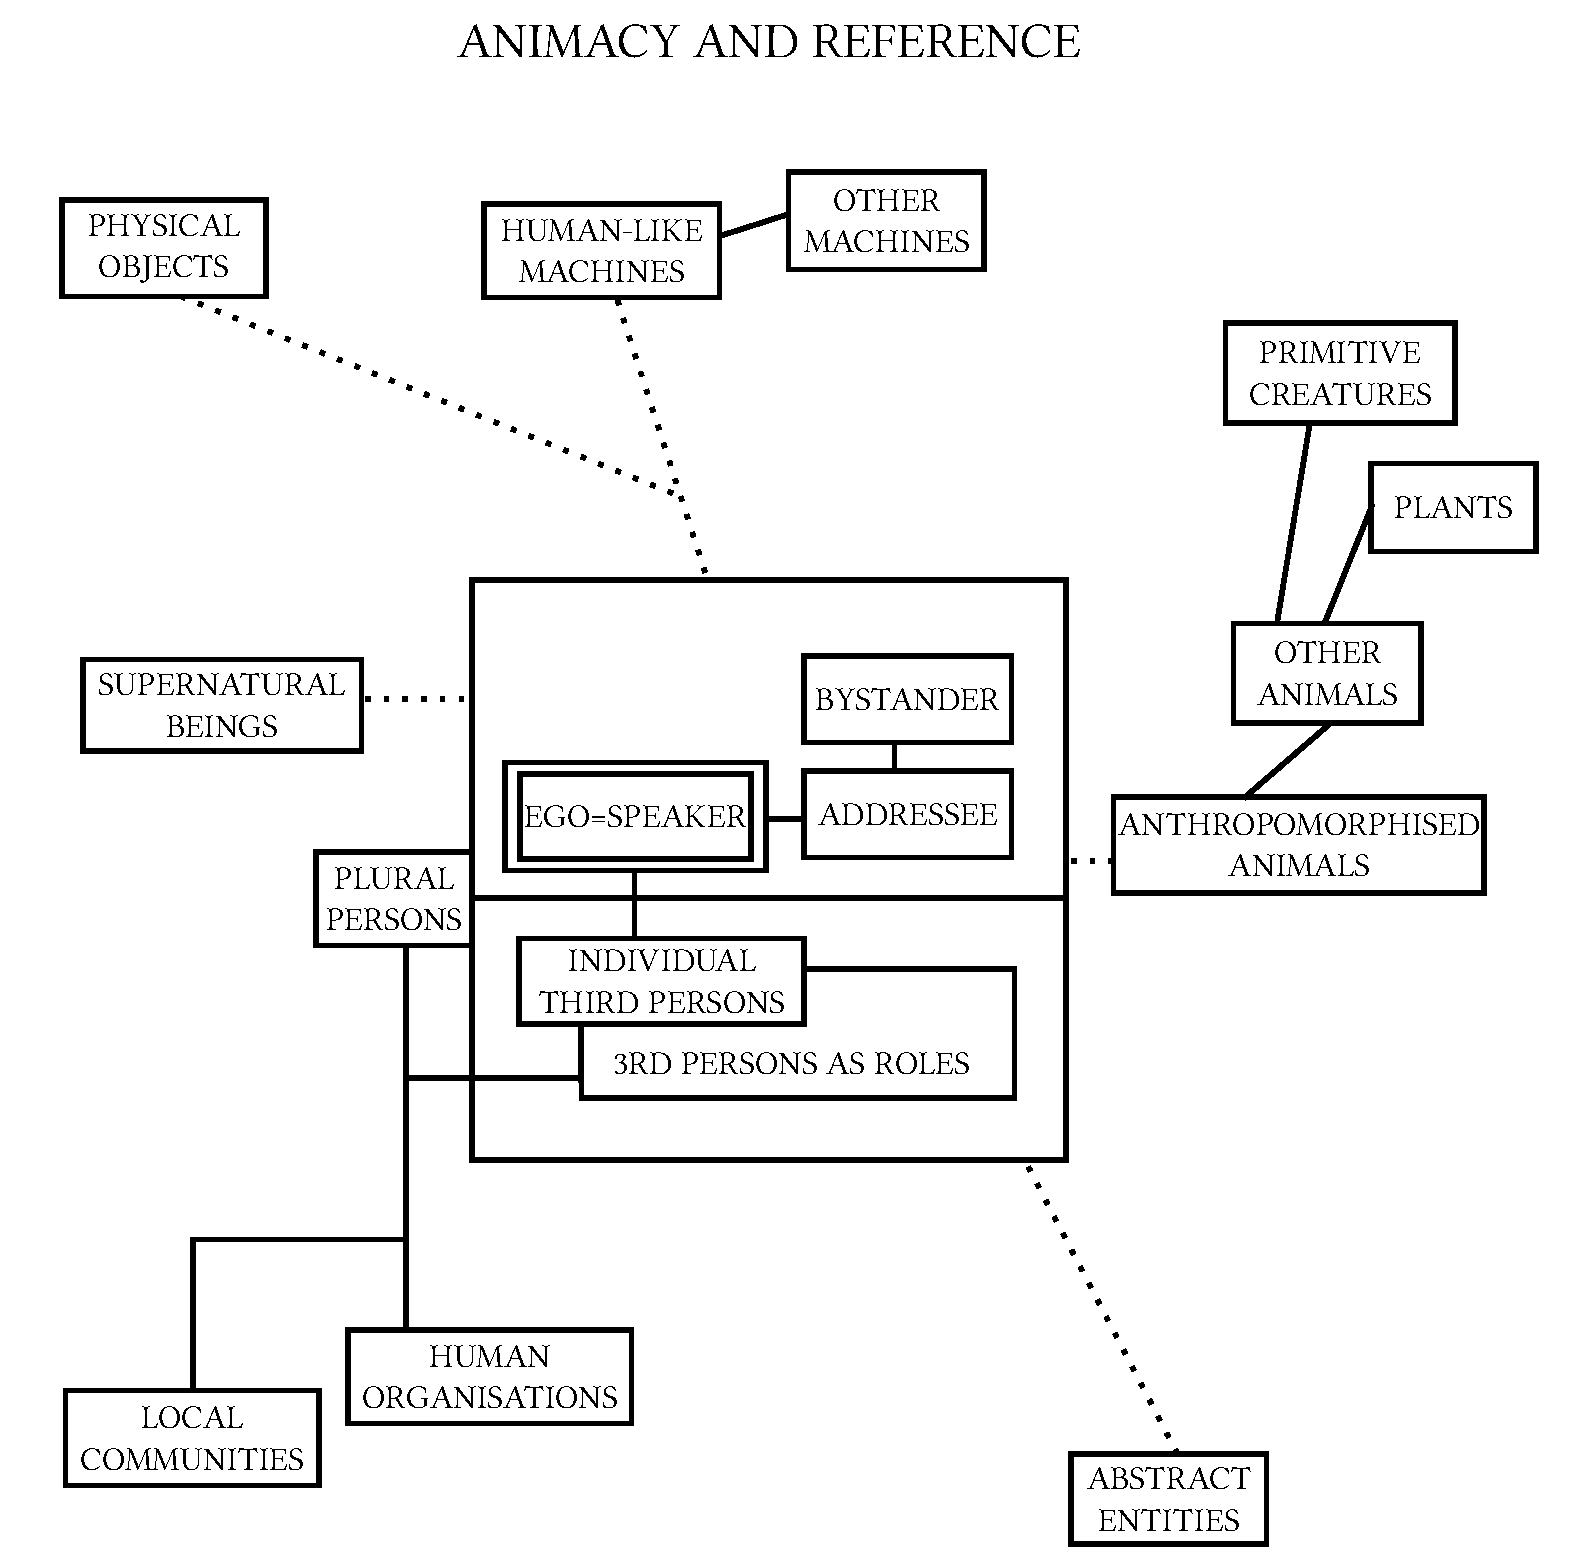
\includegraphics[width=\textwidth]{images/yamamoto2.pdf}
\caption {Belebtheitskategorien als Prototypenmodell \parencite[][38]{Yamamoto1999}\label{yamamoto}}
\end{figure} 


Im Zentrum des Prototypenmodells in Abbildung \ref{yamamoto} stehen belebte \is{Belebtheit} Entitäten, die nach Person (\textsc{Speaker, Addressee, Bystander}) und Referenzausdruck (vgl. die Skalen \ref{ex:person}  und \ref{ex:referenz} oben) weiter unterteilt sind. Nicht mehr dem prototypischen Kern zugehörig sind menschliche Referenten, die eine geringe \isi{Individualität} aufweisen, z.B. weil sie nicht alleine, sondern in der Mehrzahl agieren (\textsc{Plural Persons}) oder als Kollektiv \is{Massennomen} auftreten (\textsc{Human Organisations, Local Communities}); auf die Korrelation von \isi{Individualität} und \isi{Belebtheit} wird noch ausführlich in Abschnitt \ref{sec:indi} eingegangen. In die Peripherie gehören neben übernatürlichen Entitäten mehr oder weniger vermenschlichte Tiere und \is{Konkretum} Konkreta.  

Darüber hinaus verortet Yamamoto abstrakte Entitäten \is{Abstraktum} außerhalb des Prototypenzentrums. Eine Erweiterung der \isi{Belebtheitshierarchie}  um diese Kategorie nehmen auch \textcite{Allan1987} \textcite{Langacker1991}, und \textcite{Croft1995} vor. 

\textcite[194]{Enger2011} gruppieren zu den Abstrakta \is{Abstraktum} zusätzlich die  \object{Massennomen}, was der Skala in \REF{ex:einfachbelebt} entspricht. 

\begin{exe}
	\ex \label{ex:einfachbelebt} \textsc{human > animate > inanimate  > abstracts and massnouns}
	\end{exe}
\noindent
\isi{Massennomen} ließen sich auf den ersten Blick auch unter die unbelebten \is{Belebtheit} Konkreta \is{Konkretum} subsumieren, etwa \object{Gold}, so dass die Unbelebtheit \is{Belebtheit} allein die niedrige Platzierung auf der Skala nicht rechtfertigt. Was \isi{Massennomen} von anderen unbelebten \is{Belebtheit} Objekten wie \object{Diamant} unterscheidet, ist ihre unscharfe Kontur und damit das Kriterium der konzeptionellen Begrenztheit \parencite[203--207]{Langacker1987}. Das Gleiche gilt für Abstrakta \is{Abstraktum} wie \object{Friede}. Im Gegensatz zu \is{Konkretum} Konkreta sind sie nicht-materiell. Nach \textcite[197]{Comrie1989} differenzieren die meisten Sprachen morphologisch nicht innerhalb der Kategorie \textsc{inanimate}\footnote{Eine Ausnahme ist die Sprache der Navahos, einem Stamm Nordamerikas, in der Entitäten wie \object{Wind}, die als Verursacher einer Handlung auftreten können, durch ein spezielles Präfix von anderen unbelebten \is{Belebtheit} Objekten abgegrenzt  werden \parencite[197]{Comrie1989}, wobei man hier fragen müsste, ob eine solche Markierung nicht besser als Ausdruck der semantischen Rolle \is{Semantische Rolle} \object{Force} \parencite[73]{Primus2012} betrachtet werden sollte.}, so dass Abstrakta \is{Abstraktum} in groben Belebtheitsdistinktionen unter die Konkreta \is{Konkretum} fallen.

In Bezug auf den \isi{Definitartikel} tragen Abstrakta \is{Abstraktum} und \isi{Massennomen} allerdings eine besondere Rolle, denn sie gehören zu den Kategorien, die (im Vergleich zu quantifizierbaren \is{Konkretum} Konkreta) erst zu einer späteren Phase mit einem sich entwickelnden \isi{Definitartikel} determiniert werden, vgl. für das Althochdeutsche \textcite{Oubouzar1992} und \textcite{Szczepaniak2011}, für das Altspanische \textcite{Company1991}  oder für das Altgriechische \textcite{Napoli2009}. Auch im Gegenwartsdeutschen können sie in bestimmten Kontexten ohne Artikelwort gebraucht werden, z.B. \object{Sie kauft Gold},  \object{Wir warten auf Frieden} oder \object{Er hat Vertrag} \parencite{DAvis2013}, aber \object{*Sie kauft Haus}, \object{*Wir warten auf Brief}, \object{*Er hat Schreibtisch}. Aus diesen Beobachtungen lässt sich schließen, dass \isi{Belebtheit} sowie damit zusammenhängend die \isi{Individualität} zentrale Einflussfaktoren für die Ausbreitung des Definitartikels \is{Definitartikel} sind. 

\section{Belebtheitsgesteuerter Wandel des Definitartikels}\label{sec:belebtwandel}

Im Folgenden wird dafür argumentiert, dass die Entwicklung des Definitartikels \is{Definitartikel} entlang der \isi{Belebtheitshierarchie}  verläuft. Dass \isi{Belebtheit} nicht nur synchrone Variation, sondern auch diachronen Wandel determinieren kann, belegen eine Reihe von Studien \parencite[vgl. die Übersicht in][]{Enger2011}. Für das Deutsche hat \textcite{Kopcke1995, Kopcke2000a,Kopcke2000,Kopcke2005} gezeigt, dass die semantische Remotivierung der schwachen Maskulina (z.B. \object{der Matrose, des Matrosen})  durch den  Belebtheitsgrad \is{Belebtheit}  des Referenten gesteuert wurde. Die stete Abwanderung unbelebter \is{Belebtheit} Referenten aus dieser Deklinationsklasse hat dazu geführt, dass schwache Maskulina \is{Genus} heute belebten \is{Belebtheit} Referenten vorbehalten sind. 
Auch der Stellungswandel \is{Wortstellung} des \is{Genitivattribut} adnominalen Genitivs, der die \isi{Expansion} des Definitartikels fördert (s. Abschnitt \ref{sec:genitiv}), ist belebtheitsgesteuert \parencite[215--223]{Demske2001}: NPs \is{Nominalphrase (NP)} mit unbelebten \is{Belebtheit} Referenten tendieren seit dem späten Althochdeutschen zur Nachstellung, während belebte \is{Belebtheit} Referenten noch bis ins frühe 17. Jh. pränominal \is{Wortstellung} erscheinen (etwa: \object{des Fürsten Gewand}). Im Gegenwartsdeutschen werden hingegen in erster Linie Eigennamen \is{Eigenname} und damit typischerweise menschliche Referenten vorangestellt  (\object{Pauls Auto}).   

Die Entwicklung der satzinternen Großschreibung \parencite{Bergmann1998a,Bergmann1998,Bergmann1999,Szczepaniak2011,Szczepaniak2016} ist ein weiteres Beispiel für belebtheitsgesteuerten Wandel. Wie die Abbildung in \ref{sgs} zeigt, exponiert die Majuskel zu Beginn vor allem belebte \is{Belebtheit} und stark individuierte \is{Individualität} Entitäten (insbesondere Personennamen) und erfasst erst zum Ende des 16. Jh. regelmäßig unbelebte \is{Belebtheit} \is{Konkretum} Konkreta. Abstrakta \is{Abstraktum} werden erst Ende des 17. Jh. in der großen Mehrheit großgeschrieben.   

\begin{figure}
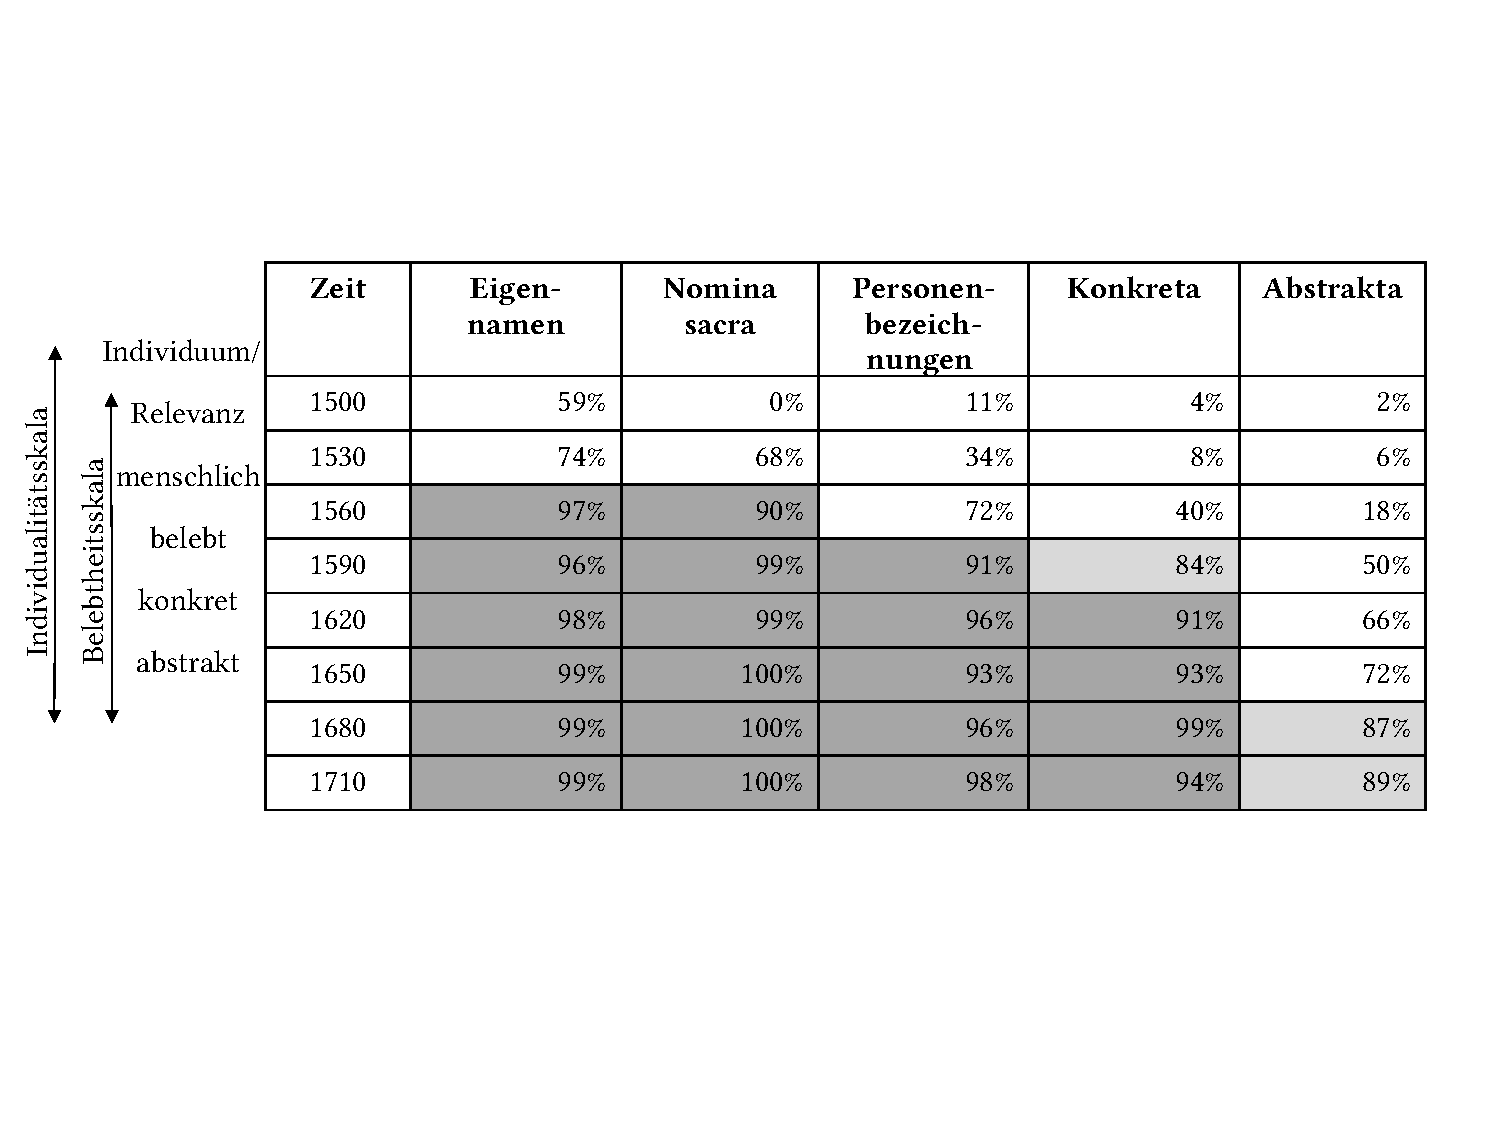
\includegraphics[width=\textwidth]{images/Substantivgrossschreibung.pdf}
\caption {Die Durchsetzung der satzinternen Großschreibung im Deutschen (\citealt{Bergmann1999}, zitiert aus \citealt[351]{Szczepaniak2011})\label{sgs}}
\end{figure} 

Die Forschung zum \isi{Definitartikel} spricht dafür, dass die Ausbreitung des Artikels in ähnlicher Weise vonstatten ging. So dokumentiert \textcite[]{Oubouzar1992} aufbauend auf einer früheren empirischen Studie \parencite{Oubouzar1989}, dass das  Artikelwort \object{dër} am Anfang (im ahd. Isidor) ebenfalls primär bei belebten \is{Belebtheit} (und diskursrelevanten) Referenten erscheint \parencite[vgl. insbesondere][566--567]{Oubouzar1989} und erst zum Ende des Ahd. auch vermehrt Abstrakta \is{Abstraktum} erfasst \parencite[][572]{Oubouzar1989}; neben Unika \is{Unikum} und generischen \is{generisch} \is{Nominalphrase (NP)} NPs, die in Abschnitt \ref{sec:definitartikel} bereits diskutiert wurden. \textcite[73--78]{Szczepaniak2011} nimmt basierend auf diesen Beobachtungen und durch die Analyse von Stichproben aus der ahd. Sprachperiode eine belebtheitsgesteuerte \is{Belebtheit} Ausbreitung \is{Expansion} des Artikels an und zwar entlang der Kategorien \textsc{belebt > unbelebt > abstrakt}. Was allerdings bislang noch fehlt, ist eine \is{Korpuslinguistik} Korpusuntersuchung, welche die Korrelation von \isi{Belebtheit} und \object{dër}-Setzung sys"-te"-ma"-tisch offenlegt. 

In der Sprachtypologie wird zwar auf das Zusammenspiel von hohem Belebtheitsgrad \isi{Belebtheit} und \isi{Definitheit} verwiesen \parencites()()[s. z.B.][53]{Dahl1996}[][166--167]{Croft2006}.\footnote{\isi{Definitheit} kann in Kombination mit \isi{Belebtheit} beispielsweise für \object{differential object marking} (=\,DOM) sorgen \parencite{Aissen2003}. \textcite{Lyons1999} liefert hierfür eine Erklärung \parencite[ähnlich argumentiert auch][119]{Croft1995}: \blockcquote[2014]{Lyons1999}{The operation for the hierarchy in some processes (most notably object marking and verb-object agreement) has been accounted for functionally, in terms of a natural tendency for the subject or agent to be more animate and more definite than the object or patient. Deviations from this natural pattern are then marked morphologically}.}
Dies wird schon allein deutlich,  wenn man die ersten drei Kategorien der \object{Extended Animacy Hierarchy} in \REF{ex:dixon} betrachtet: \is{Personalpronomen} Pronomen in der 1. Person sind naturgemäß definit, ebenso \is{Eigenname} Eigennamen. Beide Formen referieren typischerweise auf Menschen. Dass die Ausprägung der Definitheitskategorie \is{Definitheit} selbst, d.h. die  Markierung durch einen Artikel, ein Reflex belebtheitsbedingter \is{Belebtheit} Konzeptualisierung sein könnte, wird jedoch kaum diskutiert. Eine Ausnahme ist die Arbeit von \textcite{Enger2011}, in der die Frage aufgeworfen wird, von welcher Belebtheitsklasse \is{Belebtheit} aus die Kategorie \isi{Definitheit} (in Form eines sich entwickelnden Artikelwortes\footnote{Zu weiteren Möglichkeiten, \isi{Definitheit} auszudrücken, vgl. Abschnitt \ref{sec:def-ahd}.}) ihren Anfang nimmt und über welche Kategorien die \isi{Expansion} erfolgt. Zur Beantwortung formulieren \textcite[206]{Enger2011} ein sog. \hervor{Relevance Constraint}, das nicht nur für die \isi{Definitheit}, sondern auch für die Nominalkategorien \isi{Kasus}, \isi{Numerus}  und \isi{Genus} gelten soll, s. \REF{ex:enger}. 
\begin{exe}
	\ex \label{ex:enger} Language change targets the part of the lexicon where the categories in question are most relevant for human experience.
	\end{exe}
\noindent
Das \object{Constraint} bezieht sich auf eine vertikal ausgerichtete \isi{Belebtheitshierarchie}, die in Abbildung \REF{enger} zu sehen ist und den Stufen der bereits diskutierten Skala in  \REF{ex:einfachbelebt} entspricht. 
%Pronomen kommen als mögliche Belebtheitskategorie nicht in Frage, da diese nicht durch einen Definitartikel erweiterbar sind. 

\begin{figure}[h]
\begin{center}
% 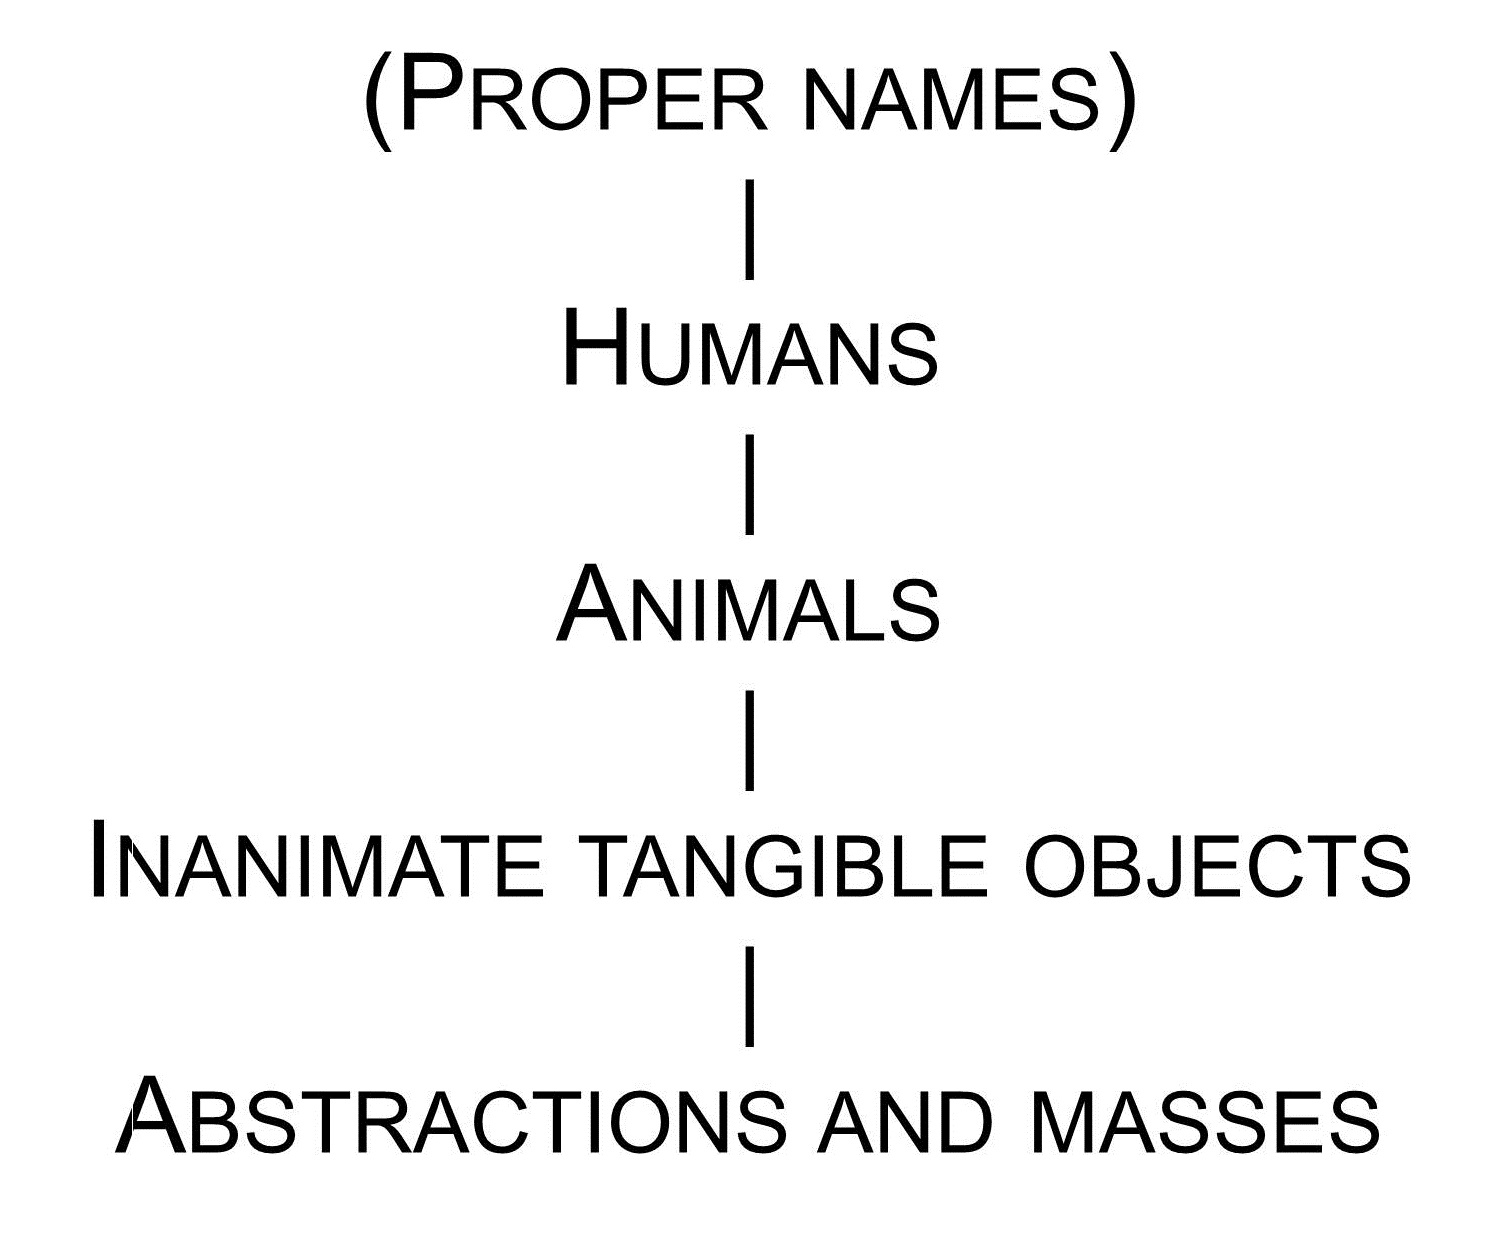
\includegraphics[width=5cm]{images/enger-hierarchie.jpg}
\begin{forest}
  [Humans
    [Animals
      [Inanimate tangible objects
       [Abstractions and masses]
      ]
    ]
  ]
]
\end{forest}
\caption {Die \isi{Belebtheitshierarchie} \parencite[194]{Enger2011}}
\label{enger}
\end{center}
\end{figure} 
Während nach \textcite[198--204]{Enger2011} \is{Numerus} Numerus- und Genusmarkierungen \is{Genus} für den Kopf der Hierarchie \is{Belebtheitshierarchie} relevant sind und Kasusmarkierungen \is{Kasus} sowohl am oberen wie am unteren Ende ihren Ursprung finden, startet \isi{Definitheit} von der Mitte der \is{Belebtheitshierarchie} Hierarchie, nämlich bei konkreten \is{Konkretum} Referenten, auf die man mit einem Gattungsnamen \is{Gattungsname} referiert.  Als Begründung führen die Autoren an, dass \isi{Definitartikel} \blockcquote[205]{Enger2011}{are used when the speaker assumes that the addressee is able to identify the referent. Since countable concrete nouns are prototypical referents, definiteness is most relevant for such nouns}. Man muss die Begründung präzisieren: Die \isi{Definitheit} ist nicht deswegen relevant, weil Konkreta \is{Konkretum} prototypische Referenten sind, sondern weil die Information identifizierbar/nicht-identifizierbar bei dieser Substantivklasse \is{Substantiv}  kommunikativ wichtig ist. Im Vergleich zu Eigennamen \is{Eigenname} wird dies besonders deutlich: Wenn ein Referent mit einem Eigennamen \is{Eigenname} denotiert wird, präsupponiert dies, dass er bekannt ist \parencite[997]{Heim2011}. Daher ist die Determinierung mit dem \isi{Definitartikel} zum Zwecke der eindeutigen \isi{Referenzierung} redundant. Der onymische Artikel \is{Eigenname} \is{Expletiver Artikel} ist aus diesem Grund erst zu einer späteren Entwicklungsstufe zu erwarten. Die Untersuchungen von \textcite{Schmuck2014} sowie \textcite{Schmuck2020} belegen den Artikelgebrauch bei Personennamen \is{Eigenname} seit dem 16. Jh. in süd-östlichen Sprachregionen. Er kommt aus pragmatischen Gründen zum Einsatz, etwa zum emphatischen Verweis oder zur Denunzierung von Referenten.

In Bezug auf das Altspanische kann \textcite[421]{Company1991} empirisch belegen, dass der \isi{Definitartikel} zuerst bei zählbaren \is{Konkretum} Konkreta, etwa \object{Spiegel} oder \object{Schwert} erscheint und begründet diese Verteilung folgendermaßen: \blockcquote[421]{Company1991}{[S]u naturaleza semántica -- ser  concretos y con límites -- era acorde
con uno de los valores del artículo, el de dar referencia, concretar y aproximar
en"-ti"-dades. (sinngemäß: \extrans{Ihre Semantik -- konkret und begrenzt zu sein -- stand in Übereinstimmung mit der Funktion des \is{Definitartikel} Artikels, nämlich zu \is{Referentialität} referieren, zu konkretisieren und Referenten in den Vordergrund zu stellen.})} Hier wird also auf die semantische Kompatibilität von Substantivklasse \is{Substantiv} und \isi{Definitartikel} verwiesen:  Wenn der \isi{Definitartikel} dazu gebraucht wird, einen Referenten von anderen potentiellen Referenten kognitiv abzugrenzen, dann ist ein solcher Abgrenzungsprozess besonders für außersprachliche Entitäten geeignet, die von sich aus eine scharfe Kontur haben und gegenständlich sind.

Im frühen Stadium seiner Entwicklung hat der \isi{Definitartikel}, wie \textcite{Epstein1993,Epstein1994} am Beispiel des altfrz. \object{le/la} zeigt, zudem die Funktion, Diskursreferenten pragmatisch hervorzuheben. Hierfür kommen vor allem menschliche Referenten in Frage, da sie wegen ihrer ontologischen Eigenschaften häufig eine besondere Hervorhebung verdienen: Sie sind kognitiv auffälliger als unbelebte \is{Belebtheit} Referenten und treten häufig als Agens \is{Agentivität} in Erscheinung, was ihre kommunikative \isi{Relevanz} für die Diskursteilnehmer erhöht. Die Auszeichnung von Menschen mit einem Artikelwort steht im Dienste der Expressivität, die auch für andere Sprachwandelprozesse, etwa den Negationswandel \parencite{Jager2008}, eine Triebfeder ist: Die Information, dass ein Referent eine hohe Diskursprominenz hat, soll möglichst deutlich markiert werden. Ein genuin demonstratives Artikelwort \is{Demonstrativartikel} ist hierfür prä"-des"-ti"-niert (vgl. hierzu auch die Ausführungen in Abschnitt \ref{sec:kata}).

Menschen bzw. konkrete \is{Konkretum} Referenten bilden also -- so die Hypothese -- den Startpunkt der Artikelentwicklung, während die Klasse der Abstrakta \is{Abstraktum} und \isi{Massennomen} undeterminiert bleiben. \textcite{Epstein1994} begründet diese Situation im Rahmen der kognitiven Linguistik folgendermaßen: \blockcquote[71]{Epstein1994}{Concrete count nouns tend to be construed as definite more frequently than
abstract or mass nouns, which are more likely to be construed as generic.
These tendencies are not surprising, given that concrete count nouns represent
entities that are cognitively more salient than abstract nouns and more
easi"-ly individuated than mass nouns. These entities are therefore more
like"-ly to be construed as referential, as active participants in a scene, and as figure rather than ground. Conversely, since abstract and mass nouns have
a lower degree of individuation, they are more likely to be construed as
non-referential, background entities.} 

Der konzeptionelle Unterschied zwischen den Substantivklassen \is{Substantiv} ist nach Epstein also eine Frage der \object{\isi{Individualität}}. Man kann die Hypothese aufstellen, dass Referenten, die von sich aus einen hohen Individualitätsgrad \is{Individualität} aufweisen,  besonders affin gegenüber einer Kennzeichnung mit dem \isi{Definitartikel} sind, weil dieser selbst einen individualisierenden Effekt auf Referenten hat. Ein Belebtheitsmodell, das die Expansionsschritte \is{Expansion} des Definitartikels \is{Definitartikel} abbilden soll, muss also über die Hierarchie \is{Belebtheitshierarchie} \textsc{menschlich > belebt > unbelebt} hinausgehen und Parameter der \isi{Individualität} mit einbeziehen. 

\section{Belebtheit und Individualität}\label{sec:indi}

Die \isi{Individualität}  erfasst, inwiefern ein Objekt sich von seiner Umgebung und anderen Entitäten abgrenzt und somit als Individuum \is{Individualität} wahrgenommen wird \parencite{Timberlake1975,Timberlake1977, Hopper1980,,Fraurud1996, Szczepaniak2011}. Die Kennzeichnung mit einem Eigennamen \is{Eigenname} ist die einfachste Art, einen hohen Individualitätsgrad \is{Individualität} zu sichern, weswegen Menschen als prototypische Individuen obligatorisch einen Eigennamen \is{Eigenname} tragen \parencite[71]{Fraurud1996}. Prinzipiell können aber auch nicht menschliche  oder sogar abstrakte Entitäten \is{Abstraktum} mittels Eigennamen \is{Eigenname} individuiert \is{Individualität} werden, etwa Haus\-tiere oder Puppen, aber auch Autos und Küchengeräte\footnote{\url{https://www.chefkoch.de/forum/2,22,447655/Haben-eure-Kuechengeraete-Namen.html}; zuletzt aufgerufen am 21.02.2020.} oder Sturmtiefs \parencite{Nubling2012}. Daran wird deutlich, dass \isi{Individualität} und \isi{Belebtheit} orthogonal zueinander laufen. In Bezug auf die für den \isi{Definitartikel} relevanten Gattungsnamen \is{Gattungsname} lässt sich allerdings zeigen, dass hohe \isi{Belebtheit} mit hoher \isi{Individualität}  korreliert: Menschen als typische Agens \is{Agentivität} beanspruchen einen größeren Handlungsraum und aktivieren ein im Vergleich zu unbelebten \is{Belebtheit} Dingen höheres Maß an Empathie \parencite{Langacker1991}. Dies macht sie zu kognitiv auffälligen Entitäten, was der \isi{Individualität}  förderlich ist. Daneben gibt es noch weitere Parameter, die einen Einfluss auf die \isi{Individualität}  haben, s. Tabelle~\ref{tab:indi}. Sie bedingen sich zum Teil gegenseitig: So sind Eigennamen \is{Eigenname} immer referentiell \is{Referentialität} und \is{Definitheit} definit\footnote{Eine Ausnahme sind Gattungslesarten \is{Gattungsname} von Eigennamen \is{Eigenname} wie in \object{Einen Schweinsteiger gibt es nur einmal}.} und nur Entitäten, die zählbar sind, können auch eine Numerusopposition \is{Numerus} aufweisen. 

\begin{table}[h]
\begin{tabular}{ll}
\lsptoprule
Individuiert & Nicht-individuiert\\ \midrule
Eigenname                    & Gattungsname         \\
Mensch, belebt               & unbelebt             \\
konkret                      & abstrakt             \\
Singular                     & Plural               \\
zählbar                      & nicht zählbar        \\
referentiell, definit        & nicht-referentiell   \\ \lspbottomrule
\end{tabular}
\caption{Faktoren für die \isi{Individualität}  \parencite[253]{Hopper1980}\label{tab:indi}}
\end{table}

Die tabellarische Einteilung geht ursprünglich zurück auf \textcite{Timberlake1975,Timberlake1977} und wird vor allem als Maß für Transitivitätseffekte \is{Transitivität} genutzt, wobei ein individuiertes \is{Individualität} Objekt \is{Objekt} die \isi{Transitivität} eines Satzes erhöht \parencite[s. auch][]{Gillmann2016}. Je mehr Eigenschaften ein Objekt aus der linken Spalte von Tabelle \ref{tab:indi} aufweist, umso näher kommt es dem prototypischen Individuum. 
Die Beispiele in \REF{ex:stossen} illustrieren das Zusammenspiel von Belebtheit, \isi{Individualität}  und \isi{Transitivität}; sie gehen zurück auf \textcite[253]{Hopper1980} und daran anknüpfend \textcite[344]{Szczepaniak2011}.

\begin{exe}
	\ex \label{ex:stossen}
	\begin{xlist}
		\ex \label{ex:stuhl} Ich stieß gegen den Stuhl.
 		\ex \label{ex:kundin} Ich stieß gegen die Kundin.
		\ex \label{ex:chalie} Ich stieß gegen Charlie.
	\end{xlist}
\end{exe}
\noindent
In \REF{ex:stuhl} liegt die Aufmerksamkeit auf dem Agens \is{Agentivität} \object{ich}. Man geht nicht davon aus, dass das (unbelebte) \is{Belebtheit} Patiens \object{Stuhl} \is{Semantische Rolle} beim  Zusammenstoß Schaden genommen hat; der Stuhl wurde nur minimal affiziert. Der Transitivitätseffekt \is{Transitivität} ist in \REF{ex:kundin} viel höher. Es ist wahrscheinlich, dass \object{der Kundin} ebenso wie dem Verursacher beim Zusammenstoß etwas passiert ist. Die Empathie und damit auch die \isi{Individualität}  steigt bei Menschen, die bekannt sind und deswegen mit einem Eigennamen ausgestattet werden können, vgl. \REF{ex:chalie}.

Nachfolgend werden die Kategorien aus Tabelle~\ref{tab:indi} erläutert und Korrelationen zum Definitartikelgebrauch \is{Definitartikel} offengelegt. 

\subsection{Der Definitartikel als \hervor{Individualisierer}} \label{sec:individualisierer} 

Unter der Opposition \object{referentiell, definit} vs. \object{nicht-referentiell} \is{Referentialität} \is{Definitheit} verstehen \textcite{Hopper1980} den Grad der Identifizierbarkeit eines Referenten und den damit verknüpften sprachlichen Mitteln. Der \isi{Definitartikel} als Marker für Identifizierbarkeit sorgt dafür, dass ein Referent an \isi{Individualität}  gewinnt -- im Gegensatz zum \isi{Indefinitartikel} --, s. \REF{ex:Referentialität}. Entsprechend kann ein \isi{Massennomen} durch den \isi{Definitartikel} eine individualisierte Lesart \is{Individualität} erhalten, wie \textcite[253]{Hopper1980} an den Beispielen in \REF{ex:bier} (hier übersetzt aus dem Englischen) illustrieren \parencite[vgl. auch][257]{Leiss2000}.

\begin{exe}
	\ex \label{ex:Referentialität} Ich habe einen/den Film gesehen.
	\ex \label{ex:bier} Fritz trank ein wenig/das Bier.
\end{exe} 
\noindent
Bei Objektinkorporierungen \is{Objektinkorporierung} liegt immer ein nicht-referentieller \is{Referentialität} Gebrauch des Substantivs \is{Substantiv} vor, s. \REF{ex:rad}; vgl. u.a. \textcite{Mithun1984}. Der \isi{Definitartikel} hebelt diese Lesart aus, indem er eine eindeutige \isi{Referenzierung} erzwingt und eine Inkorporierung blockiert, s. \REF{ex:dasrad}.  Einen ähnlichen Effekt kann man bei unspezifischen \is{Spezifizität} Nominalphrasen \is{Nominalphrase (NP)} beobachten, s. \REF{ex:unspez}. Die Auflösung der speziellen Klise \is{Klitikon} in \REF{ex:schule}, führt dazu, dass der Referent als eine bestimmte \object{Schule} identifiziert und damit individualisiert wird, s. \REF{ex:dieschule}. Wie \textcite[169]{Croft2006} zeigt, sind es sprachübergreifend in erster Linie unbelebte \is{Belebtheit} Referenten, die inkorporiert \is{Objektinkorporierung} werden, so dass Nicht-Referentialität \is{Referentialität} sowohl mit Definitheit als auch mit \isi{Belebtheit} negativ korreliert.

\begin{exe}
	\ex \label{ex:inkorp}
	\begin{xlist}
		\ex[]{\label{ex:rad} Sie fährt Fahrrad.}
		\ex[?]{\label{ex:dasrad} Sie fährt das rote Rad.}
	\end{xlist}
	\ex \label{ex:unspez}
	\begin{xlist}
		\ex[]{\label{ex:schule} Er geht noch zur Schule.}
		\ex[]{\label{ex:dieschule} Sie geht noch zu der Schule, die...}
	\end{xlist}
\end{exe} 

\noindent
Wenn der \isi{Definitartikel} selbst eine individualisierende Funktion hat, ist es wahrscheinlich, dass ein hoher Individualitätsgrad Individualität die Definitartikelsetzung \is{Definitartikel} begünstigt. Neben der \isi{Belebtheit} sind es der Konkretheitsgrad  \is{Konkretum} \is{Abstraktum} (\object{konkret-abstrakt}), der \isi{Numerus}  (\object{Singular-Plural}) und die Zählbarkeit (\object{zählbar-nicht zählbar}), die 
die \isi{Individualität}  determinieren, vgl. Tabelle~\ref{tab:indi}.

\subsection{Konkreta vs. Abstrakta}\label{sec:konabst}

Konkrete \is{Konkretum} Entitäten (etwa \object{Studentin, Hund, Kuchen}) weisen typischerweise klare Konturen auf und sind empirisch wahrnehmbar. Durch ihre Materialität grenzen sie sich maximal von ihrer Umwelt ab \parencite[344]{Szczepaniak2011}. Im Gegensatz dazu sind Abstrakta (z.B. \object{Treue, Glück}) nicht-materiell und haben keine scharfe Kontur. Es sind Einheiten, deren Bedeutung erst durch einen Abstraktionsprozess zustande kommt \parencite[279]{Ewald1992}. Weil Kinder diese Abstraktionsfähigkeit erst erlernen müssen, erwerben sie Wörter für Abstrakta \is{Abstraktum} später als Wörter für konkrete \is{Konkretum} Referenten \parencite[396]{Bergelson2013}. Die konzeptionellen Unterschiede zwischen Konkreta \is{Konkretum} und Abstrakta \is{Abstraktum} werden auch durch Studien aus der Kognitions- und Neurowissenschaft gestützt. Primingexperimente zeigen, dass beim Prozessieren von konkreten \is{Konkretum} Referenten partiell andere Hirnareale aktiviert werden als bei abstrakten \is{Abstraktum} Stimuli \parencite{Binder2005,Weiss2013}; Aphasien beeinträchtigen kognitive Funktionen wie Memorieren und Wiederholen bei Abstrakta \is{Abstraktum} stärker als bei \is{Konkretum} Konkreta \parencite{Moss1995,Moss1997}.

Die Duden-Grammatik gibt einen guten Überblick über typische abstrakte Entitäten \is{Abstraktum} und ihre Hyperonyme, s. \REF{ex:abstrakta} aus \textcite[146--147]{Duden2009}; Weitere Beispiele zu diesen Gruppen liefert \textcite[143]{Schrauf2011}.

\begin{exe}
	\ex \label{ex:abstrakta}
	\begin{xlist}
		\ex \label{ex:vorstellung} Menschliche Vorstellungen: \object{Geist, Seele}
		\ex \label{ex:handlungen} Handlungen: \object {Schlag, Wurf, Schnitt, Boykott}
		\ex \label{ex:vorgang} Vorgänge: \object{Leben, Sterben, Schwimmen, Schlaf, Reise}
		\ex \label{ex:zustand} Zustände: \object{Friede, Ruhe, Angst, Liebe, Alter}
		\ex \label{ex:eigenschaft} Eigenschaften: \object{Würde, Verstand, Ehrlichkeit, Krankheit, Länge} 
		\ex \label{ex:verhaeltnise} Verhältnisse oder Beziehungen: \object{Ehe, Freundschaft, Nähe, Unterschied}
		\ex \label{ex:wissenschaft} Wissenschaften und Künste: \object{Biologie, Mathematik, Musik, Malerei}
		\ex \label{ex:zeit} Maß- und Zeitbegriffe: \object{Meter, Watt, Gramm, Jahr, Stunde, Mai}
	\end{xlist}
\end{exe} 

Versucht man die Dichotomie \object{konkret-abstrakt} \is{Konkretum} \is{Abstraktum} auf den Substantivwortschatz \is{Substantiv} anzuwenden, stößt man schnell auf Abgrenzungsprobleme. So findet man den für Abstrakta \is{Abstraktum} definitorischen Prozess der Abstraktion auch bei \is{Konkretum} Konkreta: Beispielsweise liegt \object{Kleidungsstück} auf einer höheren Abstraktionsstufe als \object{Kleid}\footnote{Auch diese Unterschiede lassen sich neurologisch nachweisen \parencite[s.][]{Ghio2013}.} \parencite[274]{Ewald1992}. Auch eine Sammelbezeichnung wie \object{Menschheit} ist das Resultat einer Abstraktion, die mit gleichzeitiger Verminderung des Be"-lebt"-heits- und In"-dividualitätsgrades einhergeht (dies wird sichtbar im Vergleich zu \object{Menschen} als alternative Gruppenreferenz). \object{Menschheit} ist aber dennoch \hervor{belebter} \is{Belebtheit} als eine Eigenschaft wie \object{Ehrlichkeit}. Deverbale Abstrakta \is{Abstraktum} wie \object{Verschmutzung} oder \object{Wurf} haben empirisch wahrnehmbare Grenzen und sind damit stärker konturiert als ein \isi{Massennomen} wie \object{Gold}. Das Prototypenmodell von \textcite[279--280]{Ewald1992} versucht Grenzfälle wie diese zu erfassen, indem auch periphere Fälle zwischen den Polen \object{konkret} \is{Konkretum} und \object{abstrakt} \is{Abstraktum} einbezogen werden; Abbildung \ref{abb:schrauf-ewald} aus \textcite{Schrauf2011} illustriert dieses Modell.  

\begin{figure}[h]
\begin{center}
% % 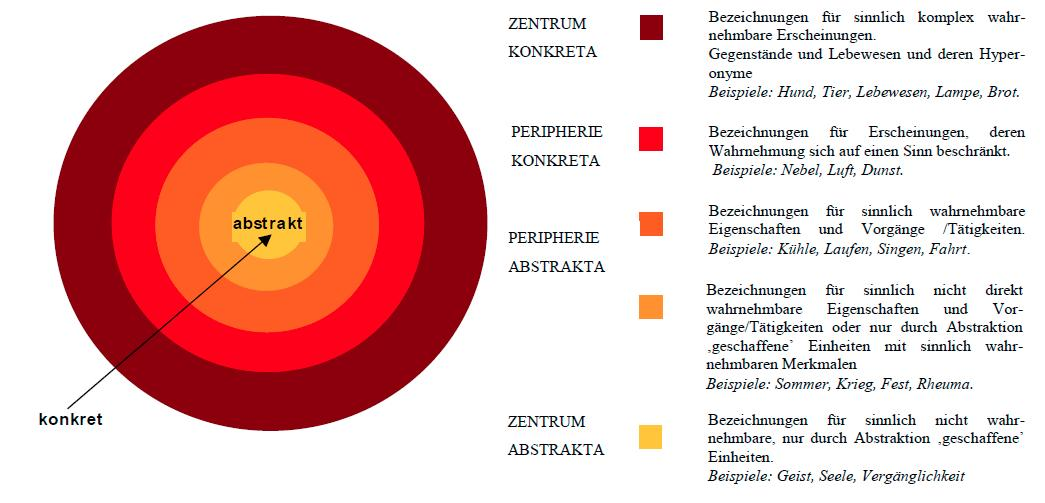
\includegraphics[width=12cm]{images/schrauff-ewald-neu.jpg}
\begin{tikzpicture}
\fill[fill=YlOrRd5] (0,0) circle (7.5em) node (outercircle) {};
\fill[fill=YlOrRd4] (0,0) circle (6em);
\fill[fill=YlOrRd3] (0,0) circle (4.5em);
\fill[fill=YlOrRd2] (0,0) circle (3em);
\fill[fill=YlOrRd1] (0,0) circle (1.5em) node (abstrakt) [font=\footnotesize] {abstrakt};
\node [below left=3cm of outercircle.south west,font=\footnotesize] (konkret) {konkret};
\draw[-{Triangle[]}] (konkret) -- (abstrakt.south);
\node [above right=2cm and 3cm of outercircle,font=\footnotesize\scshape,text width=1.5cm,align=left] {zentrum\\konkreta};
\node [above right=.25cm and 3cm of outercircle,font=\footnotesize\scshape,text width=1.5cm,align=left] {peripherie\\konkreta};
\node [below right=.25cm and 3cm of outercircle,font=\footnotesize\scshape,text width=1.5cm,align=left] {peripherie\\abstrakta};
\node [below right=2cm and 3cm of outercircle,font=\footnotesize\scshape,text width=1.5cm,align=left] {zentrum\\abstrakta};
\end{tikzpicture}\vskip2\baselineskip
{\footnotesize\begin{tabularx}{\textwidth}{@{}lQlQ@{}}
\cellcolor{YlOrRd5} & Bezeichnungen für sinnlich komplexe wahrnehmbare Erscheinungen. Gegenstände und Lebewesen und deren Hyperonyme. Beispiele: \textit{Hund}, \textit{Tier}, \textit{Lebewesen}, \textit{Lampe}, \textit{Brot}.
& \cellcolor{YlOrRd2} & Bezeichnungen für sinnlich nicht direkt wahrnehmbare Eigenschaften und Vorgänge\slash Tätigkeiten oder nur durch Abstraktion "`geschaffene"' Einheiten mit sinnlich wahrnehmbaren Merkmalen. Beispiele: \textit{Sommer}, \textit{Krieg}, \textit{Fest}, \textit{Rheuma}.\\
\cellcolor{YlOrRd4} & Bezeichnungen für Erscheinungen, deren Wahrnehmung sich auf einen Sinn beschränkt. Beispiele: \textit{Nebel}, \textit{Luft}, \textit{Dunst}.
& \cellcolor{YlOrRd1} & Bezeichnungen für sinnlich nicht wahrnehmbare, nur durch Abstraktion "`geschaffene"' Einheiten. Beispiele: \textit{Geist}, \textit{Seele}, \textit{Vergänglichkeit}.\\
\cellcolor{YlOrRd3} & Bezeichnungen für sinnlich wahrnehmbare Eigenschaften und Vorgänge\slash Tätigkeiten. Beispiele: \textit{Kühle}, \textit{Laufen}, \textit{Singen}, \textit{Fahrt}.
\end{tabularx}}
\caption {Zentrum und Peripherie bei Konkreta \is{Konkretum} und Abstrakta \is{Abstraktum} \parencite[41]{Schrauf2011}}
\label{abb:schrauf-ewald}
\end{center}
\end{figure}


\textcite{Schrauf2011} zeigt allerdings, dass Ewalds Einteilung, die partiell auf Art und Anzahl der beteiligten Sinne beruht, nicht unproblematisch ist. So kann \object{Nebel} bpsw. nicht nur visuell, sondern auch taktil oder trigeminal wahrgenommen werden. Generell basiert die Wahrnehmung meist auf dem Zusammenspiel mehrerer Sinne. Selbst periphere Abstrakta \is{Abstraktum} wie \object{Fest} enthalten Komponenten, die eindeutig sinnlich wahrnehmbar sind, z.B. \object{tanzen} oder \object{essen} etc. \parencite[vgl.][41]{Schrauf2011}. 
Eine Möglichkeit, das Modell zu ergänzen, wäre zwischen körpernahen und körperfernen Sinnen zu unterscheiden, wie es \textcite[42]{Schrauf2011} mit Bezug auf die Klassifikation von \textcite{Zimmer2007} vorschlägt, s. \REF{sinne}. \hervor{Eine definitorische Ableitung für die Konkretheitserfassung \is{Konkretum} nach diesem Modell wäre: je körpernäher der Sinn, desto konkreter} \parencite[42]{Schrauf2011}.   

\begin{exe}
	\ex \label{sinne}
	\begin{xlist}
		\ex \label{nah} Körpernahe Sinne:  taktiles, kinästhetisches, vestibuläres System, Geschmackssinn, Geruchssinn
		\ex \label{fern} Körperferne Sinne: Auditives und visuelles System
	\end{xlist}
\end{exe}

In einem von \textcite[163--166]{Schrauf2011} durchgeführten Ratingexperiment, das Wahrnehmungsunterschiede zwischen Sehenden, Blinden und nicht blinden Synästhetikern aufzeigen soll, wird deutlich, dass Lebewesen und Dinge als viel konkreter eingestuft werden als menschliche Vorstellungen (darunter \object{Bewusstsein,  Geist,  Gewissen, Gott, Hölle, Idee}) und Emotionen (u.a. \object{Angst, Ekel, Empörung, Leidenschaft, Liebe, Sicherheit, Sorge, Zweifel}), s. Abbildung \ref{abb:schrauf-rating}.\footnote{Die Abkürzung MV steht für \object{menschliche Vorstellungen}.} Die Probanden wurden gebeten, vorgegebene Kategorien auf einer Skala von 1--7 nach ihrem Konkretheitsgrad \is{Konkretum} zu bewerten. Interessanterweise erhalten gerade Lebewesen den höchsten Wert ($>6$), was dafür spricht, dass die \isi{Belebtheit} den Konkretheitsgrad \is{Konkretum} positiv beeinflusst.\footnote{Leider wird die Gruppe der Lebewesen nicht weiter in \object{menschlich} und \object{nicht menschlich} unterteilt: Die Items beziehen sich fast ausschließlich auf Tiere (z.B. \object{Fledermaus}) und Pflanzen (z.B \object{Rose}) und es werden auch \isi{Massennomen} wie \object{Geflügel} oder \object{Obst} (zur Diskussion dieser \is{Substantiv} Substantivtypen s. Abschnitt \ref{section:mass}) mit einbezogen \parencite[143]{Schrauf2011}. Der einzige menschliche Referent wird über den Ausdruck \object{Mensch} und damit einer sehr allgemeinen Kategorie erfasst.}

\begin{figure}
\begin{center}
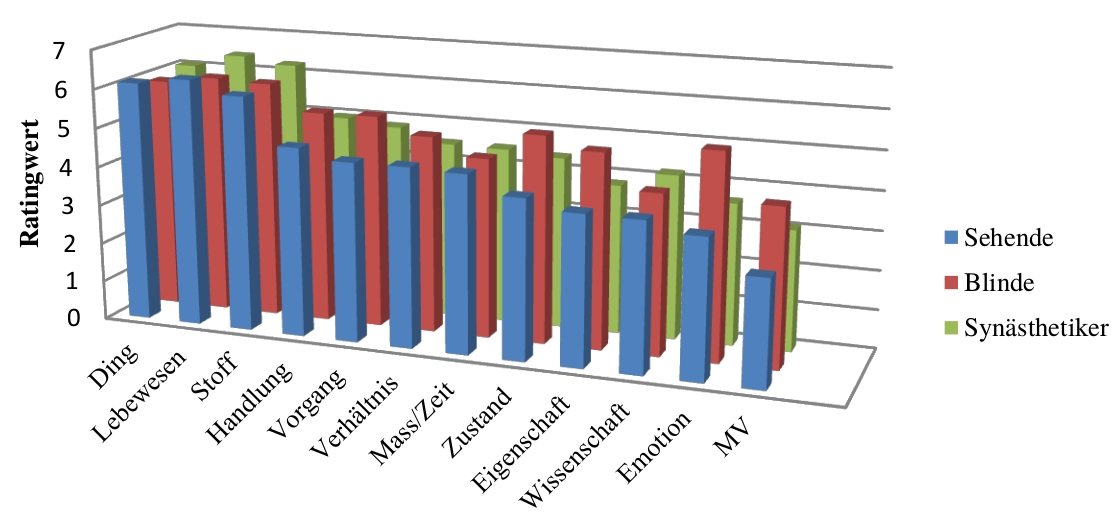
\includegraphics[width=12cm]{images/rating-konkret-abstrakt-schrauf-neu.jpg}
\caption {Ratingwerte für Konkretheit \parencite[Darstellung aus][162]{Schrauf2011}}
\label{abb:schrauf-rating}
\end{center}
\end{figure}

Für den emergierenden Artikel ist die Ausweitung von prototypischen \is{Konkretum} Konkreta in Richtung prototypische \is{Abstraktum} Abstrakta -- und damit von [+individualisiert] zu [\textminus{}individualisiert] -- zu erwarten. Eine schrittweise Kombination mit Vertretern der Peripherie kann den Weg für eine graduelle \isi{Expansion} ebnen. Wegen der Vielschichtigkeit der kognitiven Faktoren, die den Abstraktheitsgrad determinieren, wird an dieser Stelle darauf verzichtet, eine hierarchische Skala innerhalb der \hervor{untypischen} Abstrakta \is{Abstraktum} zu modellieren, die eine mögliche Expansionslinie \is{Expansion} repräsentiert. Alternativ kann man von drei Gruppen ausgehen: den Prototypen (Konkreta \is{Konkretum} und \is{Abstraktum} Abstrakta) und einem Übergangsbereich. Wie im nächsten Abschnitt gezeigt wird, ist die potentielle \object{Zählbarkeit} von Abstrakta \is{Abstraktum} und Konkreta \is{Konkretum} ein wichtiger Einflussfaktor für \isi{Individualität}  und damit eine zusätzliche Variable, die den Expansionsverlauf \is{Expansion} des Artikels innerhalb der peripheren Bereiche beeinflusst.  

\subsection{Zählbare Nomen vs. Massennomen}\label{section:mass}

Die bereits angesprochene konzeptuelle \object{Begrenztheit} ist auch zwischen zählbaren und nicht zählbaren Entitäten sowie zwischen Singular- und Pluralformen \is{Numerus} für Individualitätsunterschiede \is{Individualität} verantwortlich. Dies zeigen Studien zur sog. \object{count-mass distinction} \is{Massennomen} \parencite[s.][]{Jackendoff1991, Langacker1991, Bisle-Muller1991, Rijkhoff1991,Rijkhoff2002, Corbett2000, Massam2012,Zifonun2012}, die der Frage nach dem konzeptuellen Unterschied von zählbaren Nomen und \isi{Massennomen} nachgehen. Im Gegensatz zu Nomen wie in \REF{ex:count} sind Referenten von \isi{Massennomen} nicht zählbar und deswegen auch nicht pluralfähig \is{Numerus} \parencite[77]{Langacker1991}. Sie können sowohl konkret \is{Konkretum} als auch abstrakt \is{Abstraktum} sein, verweisen aber stets auf amorphe Referenten mit unscharfen Konturen s. \REF{ex:mass}. 

\begin{exe}
	\ex \label{ex:zaehlbarkeit}
	\begin{xlist}
		\ex \label{ex:count} Buch, Idee
 		\ex \label{ex:mass} Gold, Vernunft
 	 	\ex \label{ex:plural} Bücher, Ideen 
 			\end{xlist}
\end{exe}

\noindent
Langacker subsumiert auch die zählbaren Nomen im Plural \is{Numerus} (s. \ref{ex:plural}) unter die \isi{Massennomen}, da diese ebenfalls eine ungebundene Masse repräsentieren \parencite[77]{Langacker1991}. Die Einteilung spiegelt sich auch im grammatischen Verhalten: Beide Substantivklassen \is{Substantiv} können ohne \isi{Determinierer} eine NP \is{Nominalphrase (NP)} bilden (z.B. \object{Er will Bücher/Gold kaufen}) und lassen Quantifizierer zu, die zählbare Nomen im Singular \is{Numerus} nicht erlauben (z.B. \object{wenig Bücher/Milch}). Der Unterschied zu den \isi{Massennomen} liegt darin, dass der Plural \is{Numerus} eines zählbaren Substantivs \is{Substantiv} auch die einzelnen Bestandteile des Ganzen hervorhebt, vgl. Abbildung \ref{abb:langacker-nomen}.

\begin{figure}[h]
\begin{center}
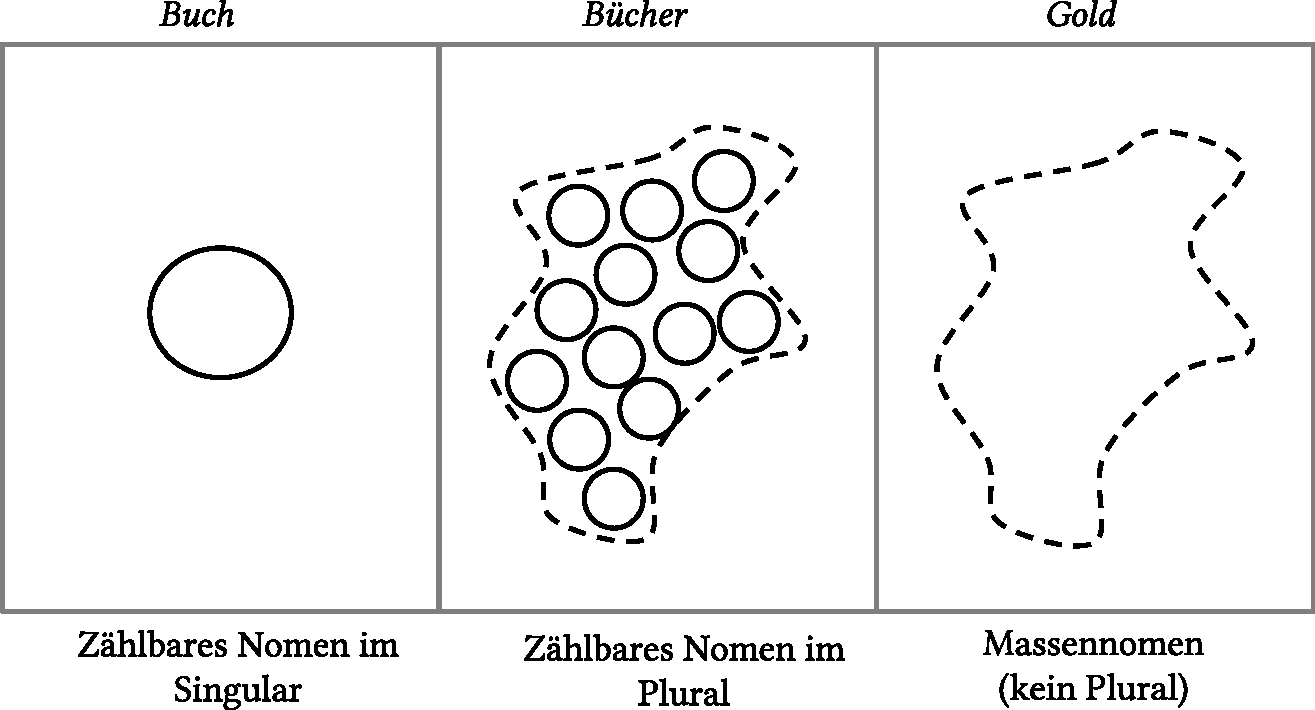
\includegraphics[width=\textwidth]{images/langacker.pdf}
\caption {Zählbare Nomen und \isi{Massennomen} im Vergleich \\ \parencite[][78]{Langacker1991}}
\label{abb:langacker-nomen}
\end{center}
\end{figure}


Die einzelnen Komponenten bei \object{Bücher} können nur deswegen profiliert werden, weil der Referent nicht aus einer homogenen Masse besteht, sondern eine \object{interne Struktur} \parencite[18]{Jackendoff1991} aus gleichen, distinktiven Einheiten besitzt. Über die Ausprägungen der Variable \object{interne Struktur} in Kombination mit \object{Begrenztheit} lassen sich Substantive \is{Substantiv} nach \textcite[20]{Jackendoff1991} in eine von vier Klassen, s. Tabelle~\ref{tab:jack} einordnen. Eine ähnliche Klassifikation nimmt \textcite{Rijkhoff1991,Rijkhoff2002} vor, indem er  unterschiedliche \object{Seinsarten} bei Substantiven \is{Substantiv} postuliert. 
Er unterscheidet \object{Shape} ($\pm$ distinktive Grenzen) und \object{Homogeneity} ($\pm$ agglomerierend).\footnote{In den Sprachen der Welt sind diese Variablen entweder unterschiedlich ausgeprägt oder unterspezifiziert, so dass man sechs Gruppen von Seinsarten annehmen kann; werden diese morphologisch markiert, spricht \textcite[121]{Rijkhoff2002} von \is{Aspekt} \object{Nominalaspekt}.}

\begin{table}
\centering
\begin{tabular}{l>{\itshape}lcc}
\lsptoprule
Substantivklasse & \multicolumn{1}{l}{Beispiel}   & Begrenztheit & Interne Struktur \\ \midrule
Individuum             & Buch       & +                                      & \textminus                                          \\
Kollektivum            & Mannschaft & +                                      & +                                          \\
Agglomerat             & Bücher     & \textminus                                      & +                                          \\
Substanz (=\,Massennomen) &   Gold       & \textminus                                      & \textminus                                          \\\lspbottomrule
\end{tabular}
\caption{Begrenztheit und interne Struktur bei Substantiven \\\parencite[20]{Jackendoff1991}}
\label{tab:jack}
\end{table}

Wegen ihrer Begrenztheit ist der Individualitätsgrad \is{Individualität} sowohl bei \isi{Massennomen} als auch bei Substantiven \is{Substantiv} im Plural \is{Numerus} geringer als bei zählbaren Substantiven \is{Substantiv} im \is{Numerus} Singular. Für Abstrakta \is{Abstraktum} wie \object{Idee} kann die Zählbarkeit eine semantische Komponente sein, die einer Determination mit einem emergierenden Artikel förderlich ist, so dass der Expansionspfad \is{Expansion} innerhalb der Abstrakta \is{Abstraktum} vermutlich von \object{zählbar} zu \object{nicht zählbar} (z.B. \object{Finsternis}) verläuft. Kollektiva \is{Massennomen} wie \object{Mannschaft} haben Referenten mit klaren Rändern, allerdings gibt es auch \is{Massennomen} Kollektiva, deren Konturen weniger scharf sind und deren interne Beschaffenheit nicht als Agglomerat von gleichen Individuen konzeptualisiert wird, sondern als Anhäufung einer homogenen Masse, was sie in die Nähe von \isi{Massennomen} bringt, etwa \object{Laub} oder \object{Vieh} \parencite[s.][120--121]{Zifonun2012}. 
Faktoren wie Größe, Auffälligkeit und \isi{Belebtheit} hängen sicherlich mit der Einteilung zusammen: Es ist wahrscheinlich, dass \object{Menschen} oder gut sichtbare Objekte wie \object{Berge} als singuläres, begrenztes Kollektiv \is{Massennomen} konzeptualisiert werden (\object{Mannschaft, Gebirge}). Dies unterstützt individualisierte Lesarten. Der kollektive \is{Massennomen} Zusammenschluss der Komponenten von \object{Laub} oder \object{Vieh} lädt hingegen zum nicht-referentiellen \is{Referentialität} und damit nicht-individualisierten \is{Individualität} Gebrauch ein (\object{Ich muss noch Laub fegen, Der Bauer hat viel Vieh}). Ein \isi{Definitartikel} kann diese Lesarten zurücknehmen und auch Referenten von \isi{Massennomen} (\object{das Laub, das Vieh, das Gold}) identifizierbar \hervor{machen}.\footnote{Der umgekehrte Fall ist ebenfalls möglich, nämlich dann, wenn der Kontext ein \isi{Massennomen} verlangt, aber ein singuläres Nomen verwendet wird, vgl. das makabere Beispiel aus \textcite[81]{Corbett2000}: \object{There was dog all over the road}.} 

Die Substantivklassifikation \is{Substantiv} aus \textcite[104]{Zifonun2012}, die im Rahmen einer Analyse zu Kompositionszweitgliedern \is{Komposition} als Ausdruck von \is{Aspekt} \object{Nominalaspekt}\footnote{Z.B.\object{-werk} als Marker für \is{Massennomen} Kollektiva, s. \textcite[101]{Zifonun2012}.} modelliert wurde, eignet sich, um  Interaktionen zwischen den genannten Individualitätskriterien \is{Individualität} zu verdeutlichen. \textcite[103]{Zifonun2012} nimmt \parencite[basierend auf den Ausführungen von][]{Rijkhoff1991,Rijkhoff2002} zwei Seinsarten für das Deutsche an, die Individuativa (=\,zählbare Nomen) und die Kontinuativa (=\,Massennomen), s. \REF{ex:seinsarten}. Orthogonal zu dieser Einteilung verläuft die Opposition konkret-abstrakt \is{Konkretum} \is{Abstraktum} sowie die Gruppe der \is{Massennomen} Kollektiva, s. Abbildung \ref{abb:zifonun-seinsarten}.

\begin{exe}
	\ex \label{ex:seinsarten}
	\begin{xlist}
		\ex \label{ex:indi} Individuativum (+Shape, \textminus{}Homogeneity)
		\ex \label{ex:konti} Kontinuativum (\textminus{}Shape, +Homogeneity)
 	\end{xlist}
\end{exe}

\begin{figure}
% % 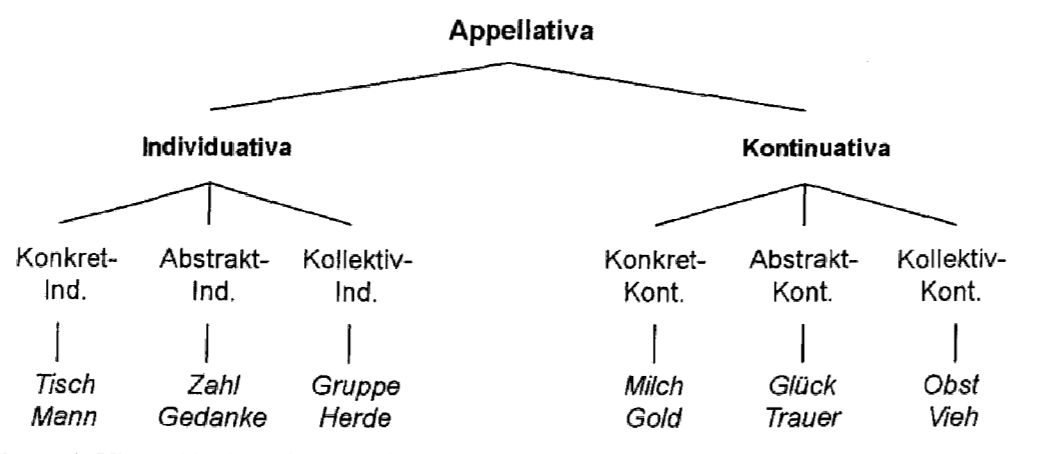
\includegraphics[width=12cm]{images/zifonun-seinarten-neu.jpg}
\begin{forest}
  [Appellativa
    [Individuativa
      [Konkret-\\Ind.,align=center   [\textit{Tisch}\\\textit{Mann},align=center] ]
      [Abstrakt-\\Ind.,align=center,before computing xy={s/.average={s}{siblings}}  [\textit{Zahl}\\\textit{Gedanke},align=center]]
      [Kollektiv-\\Ind.,align=center [\textit{Gruppe}\\\textit{Herde},align=center] ]
    ]
    [Kontinuativa
      [Konkret-\\Kont.,align=center [\textit{Milch}\\\textit{Gold},align=center] ]
      [Abstrakt-\\Kont.,align=center,before computing xy={s/.average={s}{siblings}} [\textit{Glück}\\\textit{Trauer},align=center] ]
      [Kollektiv-\\Kont.,align=center [\textit{Obst}\\\textit{Vieh},align=center] ]
    ]
  ]
\end{forest}
\caption {Seinsarten im Deutschen \parencite[104]{Zifonun2012}\label{abb:zifonun-seinsarten}}
\end{figure}

Die Eigenschaft [+Shape] sorgt für einen erhöhten Individualitätsgrad \is{Individualität} bei den Gruppenmitgliedern der Individuativa. Wenn man ein Individualitätsgefälle \is{Individualität} von Konkreta \is{Konkretum} zu Abstrakta \is{Abstraktum} annimmt, dann ist dieses Gefälle gruppenübergreifend stärker als intern, d.h. \object{Tisch} und \object{Zahl} sind wegen des Merkmals [+Shape] konzeptionell ähnlicher als \object{Tisch} im Vergleich zu  \object{Glück}. Es muss angemerkt werden, dass nach \textcite{Rijkhoff2002} ein Nomen wie \object{Gruppe} oder \object{Herde} auf der Anhäufung von Mitgliedern des gleichen Typs beruht, hier z.B. \object {Menschen} oder \object{Tiere}. Die interne Struktur solcher Nomen unterscheidet sich also gegenüber \object{einfachen} Konkreta \is{Konkretum} wie \object{Tisch}. Man müsste also eigentlich das Merkmal [+Homogeneity] vergeben.\footnote{Vgl. auch die Diskussion oben zum konzeptionell ähnlichen \object{Mannschaft}.} Als Grund, die beiden Substantivtypen \is{Substantiv} dennoch zu gruppieren, nennt \textcite[103]{Zifonun2012}  das gemeinsame grammatische Verhalten, nämlich die Fähigkeit zur Pluralbildung \is{Numerus} und die Kombinierbarkeit mit Kardinalzahlen. Sprachspezifische Kriterien wie diese können nicht ohne Weiteres auf andere Sprachsysteme übertragen werden:  Es gibt Evidenzen, dass Sprachsysteme die Grenze zwischen zählbaren und nicht-zählbaren Referenten an unterschiedlichen Stellen ansetzen: So kennt bspw. das Russische im Gegensatz zum Englischen für \object{Kartoffel} keinen \is{Numerus} Plural, wohl aber für \object{Frucht} \parencite[80]{Corbett2000}. Es stellt sich dann die Frage \blockcquote[80]{Corbett2000}{how large the component parts of a substance have to be before they are treated as individuals (for speakers of English a pea is large enough, but not for a speaker of Russian}. Interessanterweise betrifft diese Forschungsdiskussion jedoch ausschließlich unbelebte \is{Belebtheit} Referenten. Die Einteilung von Individuativnomen mit dem Merkmal [+belebt] kann deswegen auch sprachübergreifend als eigene höchst individualisierte Klasse gerechtfertigt werden. Schlägt sich die konzeptuelle Zuordnung eines Objekts in die Kategorie \object{zählbar} auch in der Grammatik nieder, so ist dies ein zusätzlicher Hinweis auf eine erhöhte \isi{Individualität} und ein Faktor, der die Determination mit Artikelwort begünstigen kann. 

\section{Belebtheit in Interaktion mit anderen Faktoren} \label{sec:andere-kog}
 
Im vorhergehenden Abschnitt wurde gezeigt, wie \isi{Belebtheit} und \isi{Individualität} zusammenhängen. Nachfolgend werden zwei weitere Faktoren besprochen, die ebenfalls mit der \isi{Belebtheit} interagieren und damit einen Einfluss auf die Artikelsetzung haben. In Abschnitt \ref{sec:partizipanten} wird auf semantische Rollen \is{Semantische Rolle} und ihre prototypische Besetzung eingegangen. In Abschnitt \ref{sec:relevanz} steht der Faktor \isi{Relevanz} im Mittelpunkt.
 
\subsection{Semantische Rollen}\label{sec:partizipanten}

Ein hoher Belebtheitsgrad \is{Belebtheit} korreliert mit bestimmten \is{Semantische Rolle} semantischen Rollen\footnote{Auch: \hervor{Partizipantenrollen} \parencite[vgl.][]{Lehmann2004a}.} \parencite[vgl. u.a.][]{Hopper1980,Comrie1989,Yamamoto2006}. So wird die Agensrolle \is{Agentivität} typischerweise mit einem Referenten besetzt, der eine Handlung willentlich ausführt oder sogar verursacht, s. Beispiele \REF{ex:agens}.

\begin{exe}
	\ex \label{ex:agens}
	\begin{xlist}
		\ex \label{ex:voll} \textit{Paul} ignoriert den Kommentar. 
 		\ex \label{ex:verursacher} \textit{Moritz} öffnet die Tür.
	\end{xlist}
\end{exe}

\noindent 
Belebte \is{Belebtheit} und insbesondere menschliche Referenten bringen die notwendigen ontologischen Eigenschaften mit, um Handlungen zu planen,  auszuführen und die Kontrolle (über ein Patiens) zu ergreifen. Traditionell wird \isi{Belebtheit} sogar als definitorisch für die Agensrolle \is{Agentivität} angesehen \parencite[16]{Primus2012}. 
Doch auch unbelebte \is{Belebtheit} Referenten sind fähig, Handlungen auszuführen, etwa im Rahmen der  Kommunikation zwischen Mensch und Maschine \parencite[s. weiterführend][18]{Primus2012}. Am mehrdimensionalen \is{Agentivität} Proto-Agens-Konzept, das von \textcite{Dowty1991} in die Forschungsdiskussion eingeführt und seither breit rezipiert wurde \parencite[vgl. u.a.][]{Ackermann2001,Primus2012,Szczepaniak2016}, wird besonders gut deutlich, dass das Merkmal \isi{Belebtheit} für einen Referenten nicht konstitutiv ist, um die Agensrolle \is{Agentivität} zu erfüllen. Es vereint sowohl die oben beschriebene prototypische \is{Agentivität} Agensrolle, als auch agens"-ähnliche \is{Agentivität} Partizipanten. Nachfolgend sind die wichtigsten Dimensionen aufgeführt, die dem Proto-Agens \is{Agentivität} zugesprochen werden  (basierend auf \citealt[572--573]{Dowty1991} und \citealt[25]{Primus2012}).  

\begin{exe}
\ex \label{ex:proto-agens}
	\begin{xlist}
        \ex  \textit{Er} hört dem Vortrag zu. (Volitionalität)
        \ex  \textit{Sie} mag Comics. (Empfindung/Wahrnehmung)
        \ex \textit{Er} zerstört den Tisch. / \textit{Rauchen} verursacht Krebs. (Verursachung)
        \ex  \textit{Sie} fiel. / \textit{Wasser} floss ins Boot. (Selbstinduzierte Bewegung)
        \ex  \textit{Sie} besitzt einige Häuser. (Besitz)
	\end{xlist}
\end{exe}

Wie \textcite[][151--152]{Yamamoto1999} hervorhebt, entspringen \isi{Belebtheit} und semantische Rollen \is{Semantische Rolle} nicht der gleichen kategorialen Ebene: Der Belebtheitsgrad  \is{Belebtheit} bezieht sich immer auf einen dem Referenten inhärenten Status. Es ist eine ontologisch begründete Klassifikation. Semantische Rollen \is{Semantische Rolle} sind hingegen relationale Begriffe, die vom Situationstyp determiniert werden, den das Verb denotiert \parencite[13]{Lehmann2004a}. Ihre Besetzung ist prinzipiell variabel: Ein belebter \is{Belebtheit} Referent wie \object{Moritz} kann bspw. sowohl als Agens \is{Agentivität} als auch als Patiens auftreten, d.h. als der von der Handlung maximal Betroffene, s. Beispiel \REF{ex:rollen}. 
 
\begin{exe}
	\ex \label{ex:rollen}
	\begin{xlist}
	 	\ex Moritz (=\,Agens) gibt Paul ein Buch.
		\ex Paul kitzelt Moritz (=\,Patiens).
 
	\end{xlist}
\end{exe}
\noindent
 
Wird ein unbelebter \is{Belebtheit} Referent personifiziert, verändert sich nicht sein \is{Belebtheit} Belebtheitsgrad, sondern seine semantische Rolle \is{Semantische Rolle} und mit ihr die Art, wie der Referent konzeptualisiert wird (vgl. \object{Die Hoffnung spricht}). 

\textcite[12]{Lehmann2004a} zufolge können belebte \is{Belebtheit} Referenten das größte Spektrum an semantischen Rollen \is{Semantische Rolle} einnehmen. Neben Agens \is{Agentivität} und Patiens sind dies Experiens, Komitativ, Emittent, Rezipient, Synpatheticus und Benefiziär.  Für Referenten, die weiter unten auf der Belebtheitsskala\footnote{\textcite{Lehmann2004a} sprechen nicht von Belebheits- sondern \is{Belebtheitshierarchie} von einer 
Empathiehierarchie, vgl. auch Abschnitt \ref{sec:belebt}.} angesiedelt sind, ist die Rollenauswahl \is{Semantische Rolle} begrenzt, doch gibt es auch hier prototypische Besetzungen. So fungieren unbelebte \is{Belebtheit} Referenten typischerweise als Instrument bzw. Force oder sie geben temporale oder lokale Relationen an \parencite[76]{Primus2012}. Letztere können auch von belebten \is{Belebtheit} Referenten ausgefüllt werden (etwa: \object{Ich gehe zum Arzt} = Ziel). 

Definitorisch für die semantischen Rollen \is{Semantische Rolle} ist die Nähe zum Situationskern, welche im Parameter Involviertheit bzw. Zentralität zum Ausdruck kommt \parencite[6]{Lehmann2004a}. Bei einer dynamischen Transitivsituation \is{Transitivität} sind bspw. Agens \is{Agentivität} und Patiens maximal involviert, weil sie konstitutiv und charakteristisch für die Handlung sind. Das Gleiche gilt für die Rolle des Rezipienten bei einer Transfersituation. Weniger zentral sind fakultative Rollen, die prinzipiell zu jeder Situation hinzutreten können, um diese zu modifizieren, d.h. u.a. temporale, lokale und kausale Rollen. Sie kommen  meist als Adverbiale \is{Adverbial} vor.

Es ist zu erwarten, dass der emergierende \isi{Definitartikel} in seiner Funktion als Individualisierer \is{Individualität} (s. Abschnitt \ref{sec:individualisierer}) bzw. Marker von Diskursprominenz (s. Abschnitt \ref{sec:kata}) zuerst bei zentralen semantischen Rollen \is{Semantische Rolle} erscheint und erst später in die \hervor{Handlungsperipherie} eindringt. Die Beobachtungen von \textcite{Himmelmann1998} stützen diese Hypothese: So sind es vor allen Dingen die \hervor{adpositional expressions} \parencite[116]{Himmelmann1998} und damit meist \is{Adverbial} Adverbiale, die in vielen Sprachen keinen \isi{Definitartikel} aufweisen. Im Gegensatz zu zentralen Partizipanten \is{Semantische Rolle} denotieren sie typischerweise Referenten, die einen niedrigen Referentialitätsgrad \is{Referentialität} haben, etwa \object{im Sommer, in Wirklichkeit, auf Erden}.  Sie dienen dazu, das Setting, in dem die Partizipanten agieren, genauer zu bestimmen \parencite["-="- orientierende Funktion, s.][118]{Himmelmann1997} und werden daher selten als Diskurstopik \is{Topik}  \is{Informationsstruktur} wiederaufgenommen. Eine besondere sprachliche Hervorhebung ist in diesen Fällen also nicht notwendig. Wahrscheinlich sorgt die zunehmende Obligatorisierung in anderen syntaktischen Kontexten dafür, dass der \isi{Definitartikel} auch die weniger zentralen Partizipanten \is{Semantische Rolle} analogisch \is{Analogie} erfasst, sofern sich die artikellose Phrase \is{Phrase} noch nicht zu sehr kognitiv eingeschliffen \is{Entrenchment} hat (zu diesem \object{Entrenchment}-Prinzip vgl. ausführlich Abschnitt \ref{sec:entrenchment}). 

\subsection{Relevanz}\label{sec:relevanz}

Die Konzeptualisierung von Objekten hängt auch mit dem Faktor \isi{Relevanz} zusammen \parencite[s.][347]{Szczepaniak2011}.  
Dieser korreliert einerseits mit der \is{Belebtheit} Belebtheit: Belebte Referenten sind relevanter als \is{Belebtheit} unbelebte, da sie  über eine höhere Handlungsgewalt verfügen und damit Einfluss auf das Denken, Handeln und Leben der Gesprächsteilnehmer haben. Anderseits ist die \isi{Relevanz} eine eigenständige Variable, deren Ausprägungen kulturell-gesellschaftlich definiert ist. Vor dem Hintergrund mittelalterlicher Hierarchiegefüge ist der König bspw. relevanter als seine Bediensteten, der Mann ist relevanter als die Frau. Im christlichen Kulturkreis genießt Gott und damit eine übermenschliche Entität, die höchste kulturelle \isi{Relevanz}. Auch Gegenstände können für Sprecherinnen und Sprecher eine erhöhte \isi{Relevanz} haben, z.B. die Bibel oder ein bestimmtes Lied. Und für Menschen in Kriegsgebieten hat das Abstraktum \is{Abstraktum} \object{Friede} sicher eine höhere \isi{Relevanz} als für Menschen, die in friedlichen Regionen wohnen.  Darüber hinaus existiert oft auch eine textuelle \isi{Relevanz}  \parencite[347]{Szczepaniak2011}: Sie gilt, wenn ein Referent besonderes eng mit dem Textthema verbunden ist oder eine zentrale Rolle für den Ausgang einer Geschichte oder die Argumentationsführung einnimmt.

Die Wirkung von \isi{Relevanz} wird bei der Entwicklung der satzinternen Großschreibung sichtbar: Im frühen 17. Jahrhundert ist die Majuskelsetzung pragmatisch gesteuert und dient u.a. dazu, religiöse Verehrung (Großschreibung von Nomina sacra) oder soziale Ehrerbietung  (Großschreibung von Titeln oder Standes- und Amtsbezeichnungen) zu markieren \parencite[73]{Bergmann1999}. Ein Beispiel für den Einfluss der textuellen \isi{Relevanz} ist die konsequente Großschreibung von \herkur{Kasten} als Synonym für die Arche Noah in der Luther-Bibel von 1534 \parencite[352]{Szczepaniak2011}. In diesem Text dominiert ansonsten die Kleinschreibung.

Auch für die Entwicklung des Definitartikels \is{Definitartikel} lässt sich postulieren: Je höher der \is{Relevanz} Relevanzgrad, desto wahrscheinlicher ist es, dass der emergierende \isi{Definitartikel} gesetzt wird. Belebte \is{Belebtheit} und kulturell wichtige Referenten sind von sich aus weit oben auf der Relevanzsskala \is{Relevanz} angesiedelt, so dass bei ihnen eine frühe Hervorhebung zu erwarten ist. 
Doch das Relevanzprinzip \is{Relevanz} kann auch bei anderen Referenten greifen. So zeigt \textcite[]{Epstein1993,Epstein1994} an altfranzösischen Sprachdaten, dass der sich entwickelnde Artikel pragmatisch genutzt wird, um bspw. Abstrakta, die gewöhnlich als unspezifische Entitäten konzeptualisiert werden und dann undeterminiert bleiben, in bestimmten Fällen eine eindeutig identifizierbare und diskursprominente Lesart zuzuschreiben. Dies ist in einer der frühesten Überlieferungen  (\hervor{La chanson de Roland} um 1080) zu sehen, wenn von dem Tod (\object{la mort}) oder dem Verrat (\object{la traïsun}) einer der Leserschaft bekannten Person berichtet wird \parencite[71--72]{Epstein1994}. Eine ähnliche pragmatisch gesteuerte Artikelsetzung vermutet auch \textcite[218]{Oubouzar1989} für das frühe Althochdeutsche. 

\section{Zusammenfassung} \label{sec:bel-zusammenfassung}

Aus den bisherigen diachronen Untersuchungen lässt sich die Hypothese ableiten, dass die kognitiv-linguistische Kategorie \isi{Belebtheit} den Expansionsweg \is{Expansion} des emergierenden Definitartikels \is{Definitartikel} lenkt. Der Startpunkt ist bei den belebten \is{Belebtheit} und insbesondere menschliche Referenten zu suchen, da Sprecherinnen und Sprecher diesen meist die höchste \isi{Relevanz} im Diskurs zuschreiben.
Sie sind kognitiv besonders auffällig, da sie typischerweise den größten Handlungsraum im Diskurs einnehmen. Das ursprünglich demonstrative \object{dër} \is{Demonstrativartikel} kann diese Diskursprominenz sprachlich unterstreichen. Da jede Form des Determinierens einen kognitiven Abgrenzungsprozess beinhaltet -- aus einer Menge von möglichen Referenten wird eine Teilmenge ausgewählt, wodurch andere in Frage kommende Referenten ausgegrenzt werden -- ist zu erwarten, dass Referenten mit unscharfen Grenzen, darunter \is{Abstraktum} Abstrakta, Kollektiva und Stoffe \is{Massennomen} sowie zählbare Nomen \is{Numerus} im Plural, \hervor{schlechtere} Kandidaten für eine definite Kennzeichnung sind als Referenten mit scharfen Grenzen. Zu diesen gehören \is{Konkretum} konkrete, zählbare, \is{Numerus} singulare Entitäten. Sie sind empirisch direkt wahrnehmbar, haben einen höheren Kontrast zu ihrer Umwelt und zu anderen Referenten als konturlose Objekte und sind dadurch stärker individualisiert. 

Mit zunehmender Konventionalisierung -- so die Hypothese -- verliert \object{dër} seine pragmatische Kraft und wird zum obligatorischen Marker für alle \is{Substantiv} Substantivklassen. Neben der \isi{Individualität} korreliert auch der Faktor \isi{Agentivität} mit einem hohen Belebtheitsgrad \is{Belebtheit}, weswegen dieser in das \is{Belebtheit} Belebtheitsmodell, das der nachfolgenden Untersuchung zugrunde liegt, mit einbezogen wird, vgl. Abbildung \ref{abb:belebtheit-gesamt}, die auf den Darstellungen von \textcite[345]{Szczepaniak2011} und \textcite[98]{Nubling2012} basiert.  
    
\begin{figure}
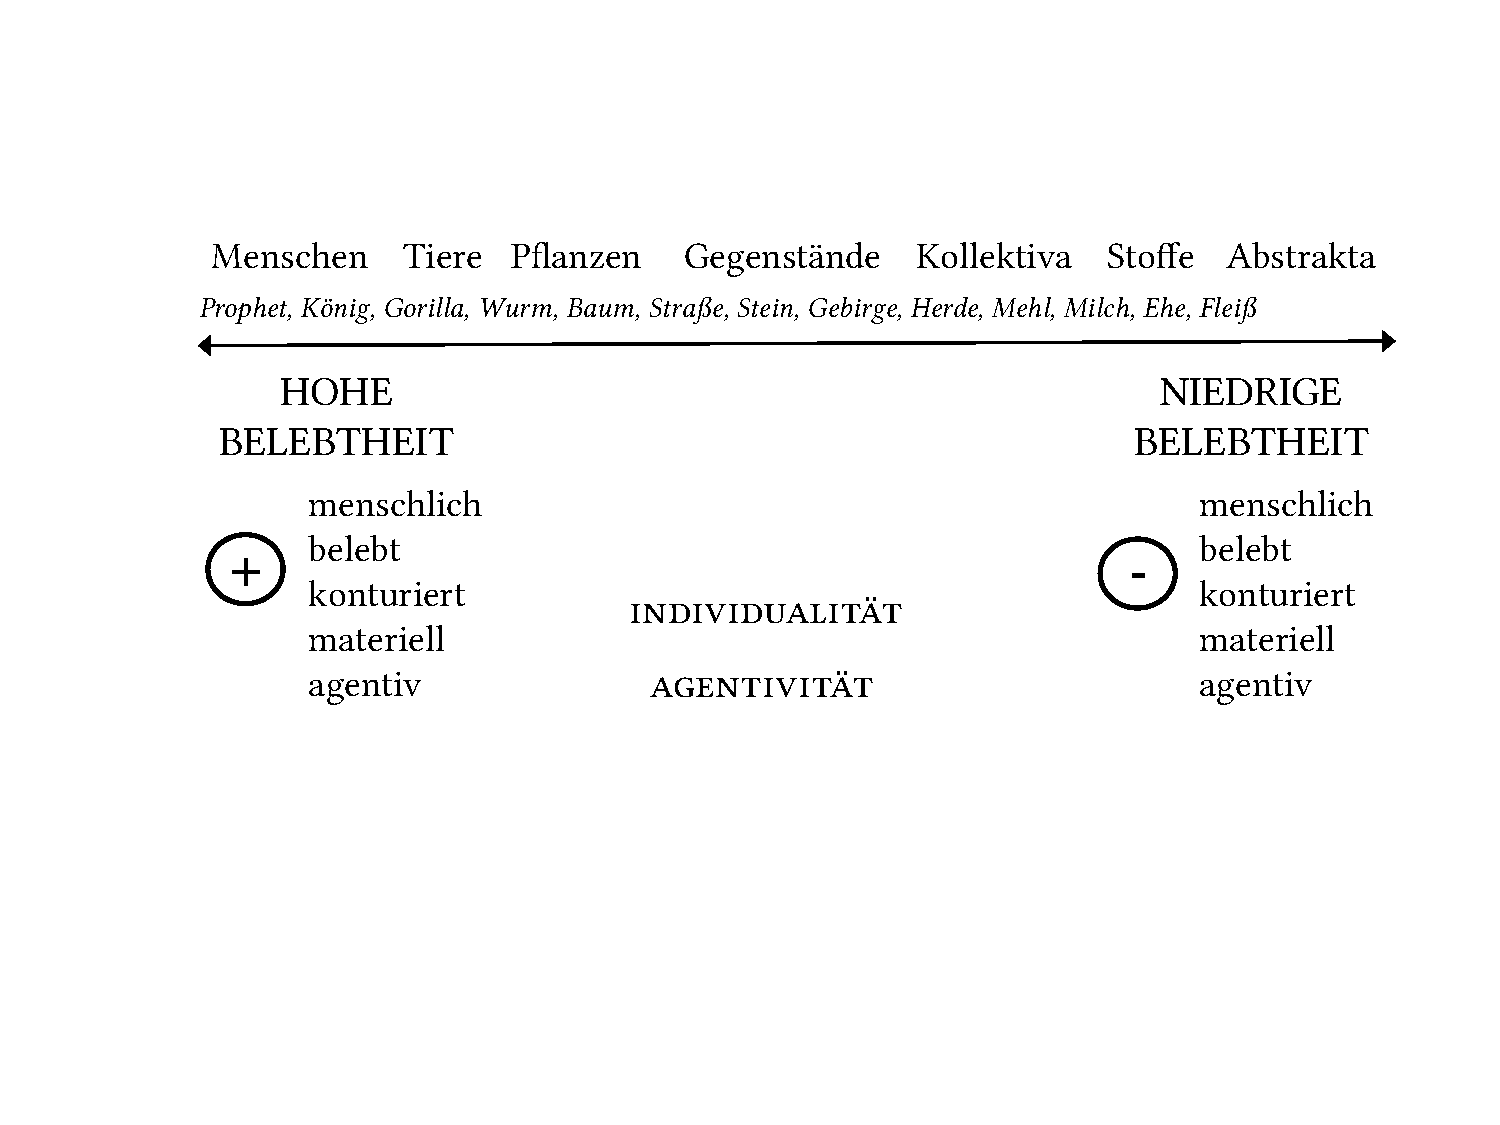
\includegraphics[width=.75\textwidth]{images/Belebtheitsshierarchie.pdf}
\caption{Belebtheit und korrelierende Faktoren\label{abb:belebtheit-gesamt}}
\end{figure}


Nicht mit in der Darstellung aufgenommen ist die Zählbarkeit und damit zusammenhängend der \isi{Numerus} eines Objekts. Diese Kriterien laufen quer zur \isi{Belebtheitshierarchie}, in dem Sinne, dass im Prinzip alle konkreten \is{Konkretum} Entitäten (also Menschen, Tiere, Gegenstände) je nach Vorkommen und Konzeptualisierung in ihrer Zählbarkeit und damit im \isi{Numerus} variieren. Für \is{Abstraktum} Abstrakta ist die Unterscheidung nicht relevant. Denn selbst zählbare \is{Abstraktum} Abstrakta wie \object{Grausamkeit} weisen keine numerusspezifischen \is{Numerus} konzeptuellen Unterschiede auf, welche die Individualität beeinflussen würden. Generische \is{generisch} Lesarten sind bei allen Referenten prinzipiell möglich, bei Referenten auf der rechten Seite des Modells allerdings wahrscheinlicher als auf der linken, so dass dies einer frühen Determinierung mit \object{dër} zusätzlich im Wege steht. Eine hohe gesellschaftlich-kulturelle und textuelle \isi{Relevanz} ist bei belebten \is{Belebtheit} Referenten zwar besonders wahrscheinlich. Je nach Kontext und Textthema ist \isi{Relevanz} aber auch ein Faktor, der bei unbelebten und \is{Abstraktum} abstrakten Referenten wirksam sein kann, so dass er orthogonal zur linearen Hierarchie verläuft. 
